\documentclass[aspectratio=169,11pt,t]{beamer}
% ============================================================
%  ksa-cs-v2: ksa-cs-lecture-template.tex 스타일 + 한글, v2 덱(16:9)용.
%    - 짙은 네이비 헤드라인 (섹션 이름 + 프레임마다 점)
%    - 꽉 찬 파란 제목 막대, 둥근 그림자 블록
%    - 한글: Noto Sans CJK KR (fontspec)
%  사용:
%    \documentclass[aspectratio=169,11pt,t]{beamer}
%    \input{<..>/theme/ksa-cs-v2.tex}
%  ksa-theme.tex 의 매크로(\kb \kq, ksablue/ksared 등)도 같은 이름으로 둔다
%  -> v2 덱 본문을 거의 그대로 옮길 수 있다.
% ============================================================

\usepackage{fontspec}
\usepackage{amsmath,amssymb}
\usepackage{tikz}
\usepackage{listings}
\usepackage{graphicx}
\usepackage{booktabs}
\usepackage{varwidth}
% enumitem 은 넣지 않는다 (beamer 글머리표가 사라진다)

\defaultfontfeatures{Ligatures=TeX}
\setmainfont{Noto Sans CJK KR}
\setsansfont{Noto Sans CJK KR}
\setmonofont{Noto Sans Mono CJK KR}[Scale=0.92]
\usefonttheme{professionalfonts}

% ---------- 기본 틀 ----------
\usetheme{default}
\useinnertheme[shadow=true]{rounded}
\setbeamertemplate{navigation symbols}{}
\setbeamersize{text margin left=1em,text margin right=1em}

% ---------- 색 (템플릿 원본 값) ----------
\definecolor{navydark}{HTML}{191959}
\definecolor{navydim}{HTML}{8888B0}
\definecolor{navytitle}{HTML}{262686}
\definecolor{navyblue}{HTML}{3333B2}
\definecolor{blockbodybg}{HTML}{E9E9F3}
\definecolor{examplegreen}{HTML}{006000}
\definecolor{examplebg}{HTML}{E5EFE5}
\definecolor{alertred}{HTML}{BF0000}
\definecolor{alertbg}{HTML}{F9E5E5}
% ksa-theme.tex 와 같은 이름 (본문 호환)
\colorlet{ksablue}{navytitle}
\colorlet{ksabluedk}{navydark}
\definecolor{ksagold}{HTML}{D6CBB1}
\definecolor{ksagolddk}{HTML}{A9976B}
\colorlet{ksared}{alertred}
\definecolor{ksagray}{HTML}{5B5B5B}

\setbeamercolor{structure}{fg=navyblue}
\setbeamercolor{alerted text}{fg=alertred}
\setbeamercolor{frametitle}{bg=navytitle,fg=white}
\setbeamercolor{title}{fg=white,bg=navytitle}
\setbeamercolor{block title}{bg=navytitle,fg=white}
\setbeamercolor{block body}{bg=blockbodybg,fg=black}
\setbeamercolor{block title example}{bg=examplegreen,fg=white}
\setbeamercolor{block body example}{bg=examplebg,fg=black}
\setbeamercolor{block title alerted}{bg=alertred,fg=white}
\setbeamercolor{block body alerted}{bg=alertbg,fg=black}
\setbeamercolor{item}{fg=navyblue}
\setbeamertemplate{itemize item}[circle]
\setbeamertemplate{itemize subitem}[triangle]

% ---------- 헤드라인: miniframes (섹션 이름 + 점) ----------
\useoutertheme[subsection=false]{miniframes}
\setbeamerfont{section in head/foot}{size=\tiny}
\setbeamercolor{section in head/foot}{bg=navydark,fg=white}
\setbeamercolor{mini frame}{fg=white}
\setbeamertemplate{mini frames}[circle]

% ---------- 제목 막대: 폭 꽉 채움, 두 줄까지 ----------
\setbeamerfont{frametitle}{size=\normalsize,series=\bfseries}
\setbeamertemplate{frametitle}{%
  \nointerlineskip
  \begin{beamercolorbox}[wd=\paperwidth,ht=2.7ex,dp=1.1ex,leftskip=.3cm,rightskip=.3cm]{frametitle}%
    \usebeamerfont{frametitle}\insertframetitle
  \end{beamercolorbox}}

% ---------- 쪽 번호: 오른쪽 아래 ----------
\setbeamertemplate{footline}{%
  \hfill
  {\color{navydim}\scriptsize\insertframenumber\,/\,\inserttotalframenumber}%
  \hspace{3mm}\vspace{2mm}%
}

% ---------- 표지: 템플릿처럼 헤드라인은 그대로, 가운데 둥근 그림자 상자에 제목 한 줄 ----------
% 덱에서:  {\setbeamertemplate{footline}{}\begin{frame}[c,noframenumbering]\titlepage\end{frame}}
\setbeamercolor{title}{fg=white,bg=navyblue}
\makeatletter
\setbeamertemplate{title page}{%
  \vfill
  \centering
  \begin{minipage}{0.84\paperwidth}
  \begin{beamercolorbox}[wd=\linewidth,sep=7pt,center,rounded=true,shadow=true]{title}
    {\usebeamerfont{title}\inserttitle\par}%
    \ifx\insertsubtitle\@empty\else\vskip0.4em{\usebeamerfont{subtitle}\insertsubtitle\par}\fi
  \end{beamercolorbox}
  \end{minipage}\par\vskip1.6em
  {\usebeamerfont{author}\color{navytitle}\insertauthor\par}\ifx\beamer@date\@empty\vskip0.3em\else\vskip1.3em\fi
  {\usebeamerfont{institute}\color{ksagray}\insertinstitute\par}%
  \ifx\beamer@date\@empty\else\vskip0.3em{\usebeamerfont{date}\color{ksagray}\insertdate\par}\fi
  \vfill
}
\makeatother
\setbeamerfont{title}{series=\bfseries,size=\Large}
\setbeamerfont{subtitle}{size=\normalsize}
\setbeamerfont{author}{size=\normalsize}
\setbeamerfont{institute}{size=\small}
\setbeamerfont{date}{size=\small}

% ksa-theme 호환: 덱이 \renewcommand{\ksacredit}{..} 를 해도 되게 (꼬리말에는 안 쓴다)
\newcommand{\ksacredit}{}

% ---------- 강조 ----------
\newcommand{\hl}[1]{\textcolor{alertred}{#1}}
\newcommand{\hlb}[1]{\textcolor{navyblue}{#1}}
\newcommand{\kb}[1]{\textbf{\color{ksablue}#1}}
\newcommand{\kq}[1]{\textbf{\color{ksared}#1}}

% ---------- 파이썬 코드 (템플릿과 같은 색) ----------
\definecolor{codekw}{HTML}{0033B3}
\definecolor{codebuiltin}{HTML}{BF0000}
\definecolor{codestr}{HTML}{067D17}
\definecolor{codecomment}{HTML}{8C8C8C}
\definecolor{codenum}{HTML}{1750EB}
\lstdefinestyle{py}{
  language=Python, basicstyle=\ttfamily\scriptsize,
  keywordstyle=\color{codekw}\bfseries, stringstyle=\color{codestr},
  commentstyle=\color{codecomment}\itshape, numberstyle=\color{codenum},
  emph={print,len,range,sum,input,int,str,float,list,dict,append,remove,sorted,abs,min,max},
  emphstyle=\color{codebuiltin}, showstringspaces=false, keepspaces=true,
  columns=fixed, basewidth=0.52em, aboveskip=1mm, belowskip=1mm, xleftmargin=2mm,
  breaklines=true
}
\lstset{style=py}

\usepackage{fontawesome5}
\newcommand{\paperlink}[1]{\href{#1}{\textcolor{ksablue}{\faLink}}}
% SVM 수업 두 덱 중 둘째 (2026-11-26 Stanford CME 250 범위로: 커널 학습·원 논문 실험은 보충 덱 ../../week02/9_svm_extra, RBF 전개 쪽은 수업에 다시 둠)
\setbeamerfont{author}{size=\normalsize}
\setbeamerfont{institute}{size=\small}
\graphicspath{{figs/}{../../../assets/}}
\usetikzlibrary{tikzmark,shapes.callouts,positioning}
\tikzset{bub/.style={draw=ksagolddk,line width=1pt,fill=ksagolddk!10,rounded corners=3pt,inner sep=4pt,font=\normalsize,align=left},
         bubarr/.style={-latex,ksagolddk,line width=1.2pt}}
\definecolor{fgap}{HTML}{1B7F3B}\definecolor{fx}{HTML}{D62728}\definecolor{fsh}{HTML}{2E3192}\definecolor{fbeta}{HTML}{7A6A3F}\definecolor{fdist}{HTML}{000000}\definecolor{fbd}{HTML}{555555}
\makeatletter
\newcommand{\markpage}[1]{\protected@write\@auxout{}{\string\newlabel{#1}{{\the\c@framenumber}{}}}\hypertarget{#1}{}}
\newcommand{\pref}[1]{\hyperlink{#1}{\textcolor{ksagolddk}{(p.\ref{#1})}}}
\makeatother

\renewcommand{\ksacredit}{Machine Learning and Deep Learning \,\textperiodcentered\, SVM 2: 커널}
\title{SVM 2: 커널 (Kernel SVM)}
\subtitle{특징 늘리기 · 커널 트릭 · RBF}
\author{Machine Learning and Deep Learning}
\institute{KSA 2027-Spring}
\date{Sumin Han (suminhan@ksa.hs.kr)}
\begin{document}
{\setbeamertemplate{footline}{}\begin{frame}[c,noframenumbering]\titlepage\end{frame}}

\section{질문}
% --- 직관 1: 스프링 · 두 자 · 못
\begin{frame}{지난 시간의 답을 다시 보면: 스프링이 벌린 두 자가 \textbf{못 3개}에 걸려 멈춘다}
\vfill
\centering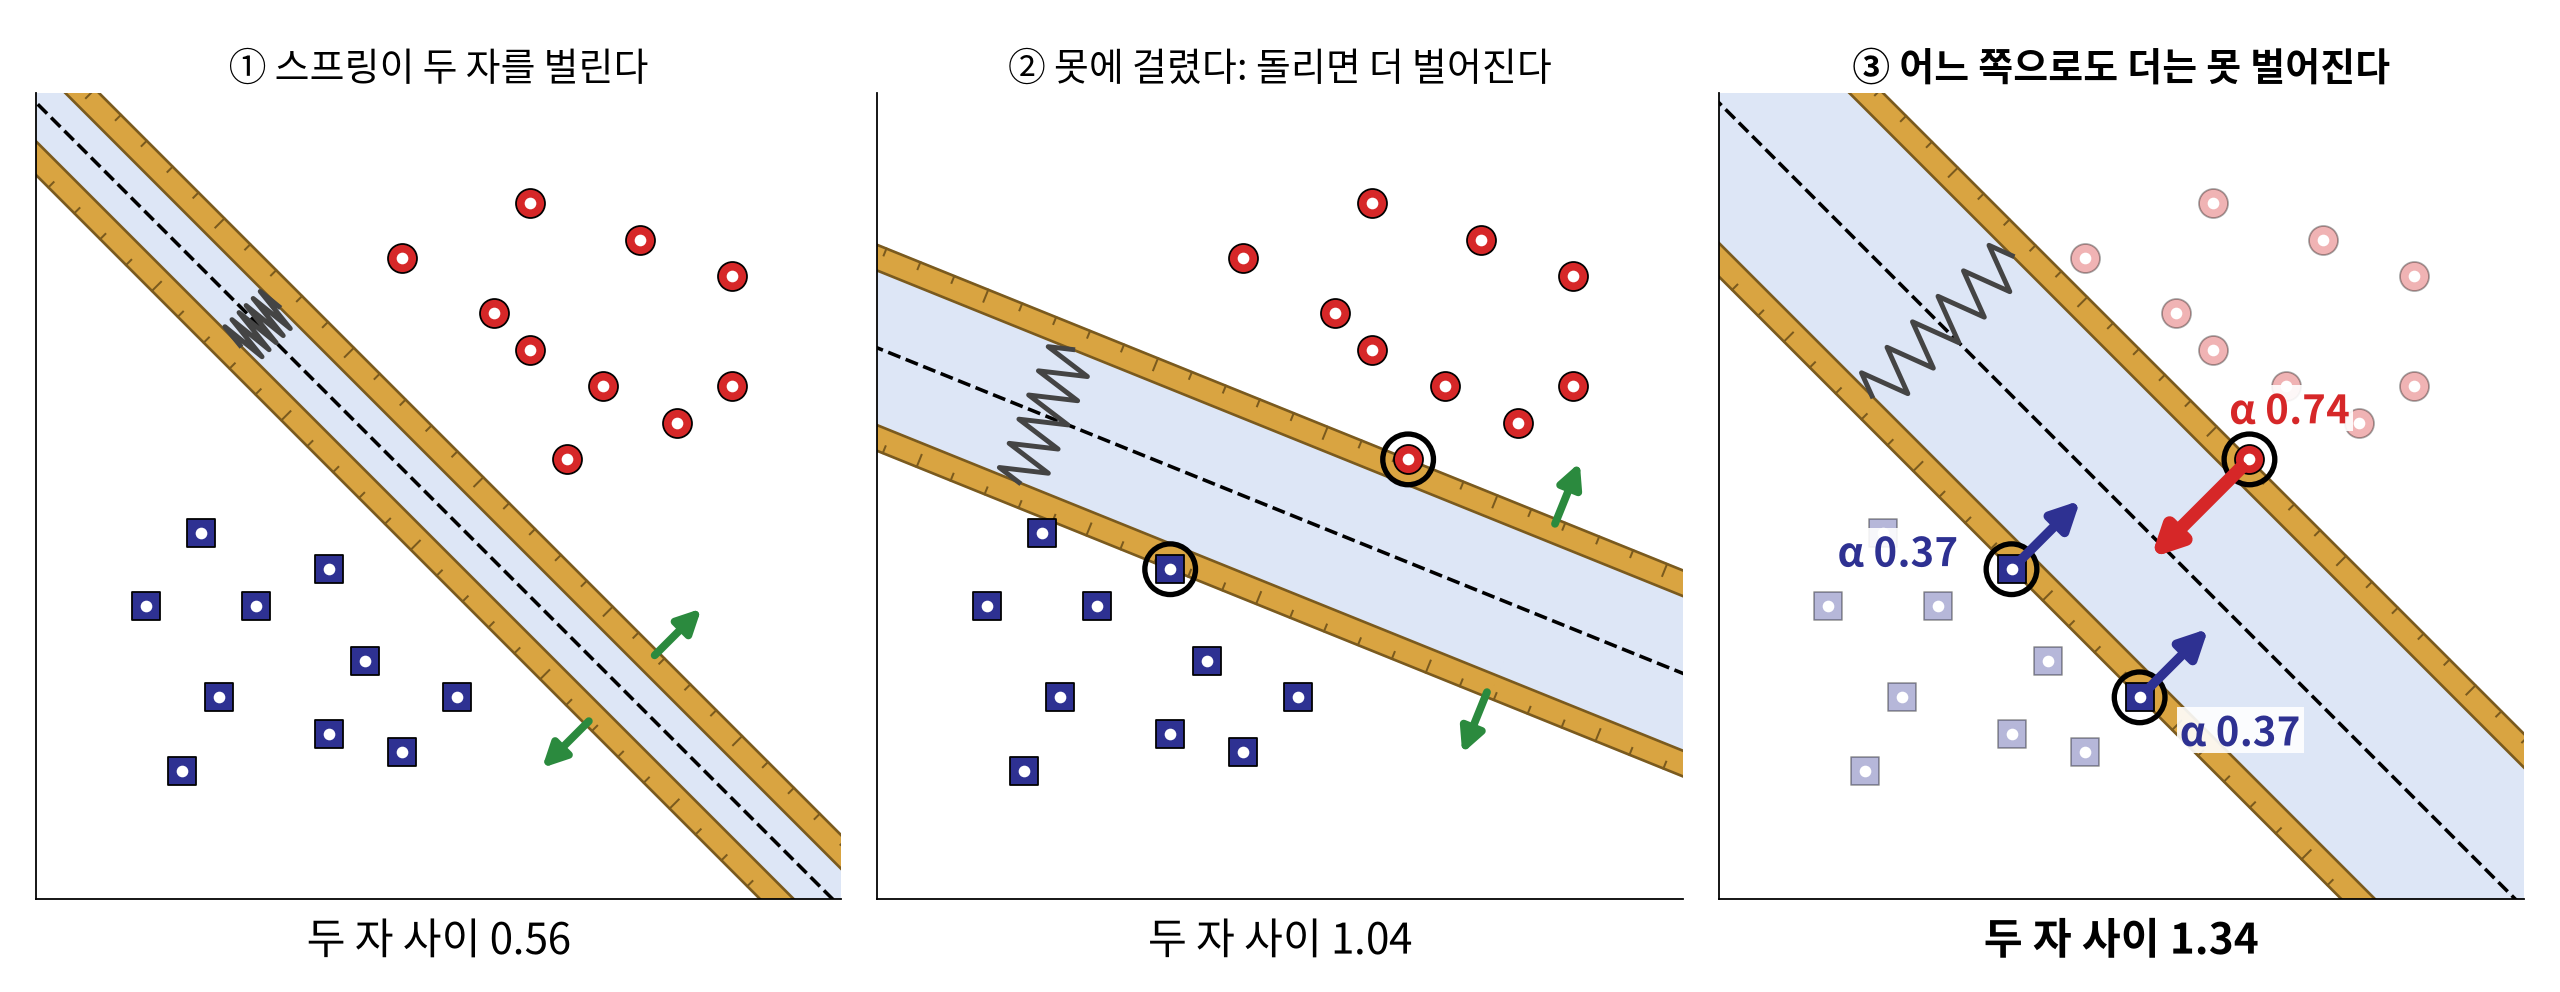
\includegraphics[width=0.70\linewidth]{kn_nails_unit.png}\par\vskip0.2em
{\large 못 = 학습 점 \;·\; 두 자 사이 = 길 폭 $2M$ \;·\; 스프링 = 길을 넓히려는 힘}\\[0.15em]
{\large 자가 닿은 못 = \kb{서포트 벡터}, 못이 버티는 힘 = \kq{$\alpha_k$} \;·\; 안 닿은 못 17개는 힘 \textbf{0}}\\[0.4em]
{\large 멈췄다 $=$ 스프링 힘 $=$ 못들이 버티는 힘의 합 \;$\to$\; \fcolorbox{fbeta}{fbeta!10}{$\mathbf{w} = \sum_k \alpha_k y_k \mathbf{x}_k$}}\\[0.1em]
{\normalsize 답의 $\mathbf{w}$ 는 언제나 이렇게 쓸 수 있도록 \textbf{$\alpha_k \ge 0$ 를 정할 수 있다} (서포트 벡터만 $\alpha_k \neq 0$)}
\vfill
\note{지난 시간의 최대 마진을 그림 하나로 다시 봅시다. 점마다 못이 박혀 있고, 두 자 사이에 스프링이 있어서 길을 계속 넓히려 합니다. 첫째 그림처럼 아무 못에도 안 닿으면 자는 계속 벌어집니다. 둘째 그림처럼 못 두 개에 걸려도, 자를 돌리면 더 벌어질 수 있습니다. 셋째 그림처럼 못 세 개에 걸리면 어느 쪽으로 돌려도 더는 못 벌어지고 멈춥니다. 이것이 최대 마진입니다. 자에 닿은 못이 서포트 벡터이고, 그 못이 자를 버티는 힘의 크기를 알파라고 부릅니다. 빨강 못이 0.74, 파랑 못 둘이 0.37씩 버티고, 자에 안 닿은 못 17개는 아무 힘도 쓰지 않으니 알파가 0입니다. 멈췄다는 것은 스프링이 미는 힘과 못들이 버티는 힘이 비겼다는 뜻입니다. 그래서 스프링 쪽인 w는 닿은 못들의 힘을 더한 것, 알파 k 곱하기 y k 곱하기 x k의 합과 같습니다. 정확히 말하면, 최대 마진의 답 w는 언제나 이렇게 쓸 수 있도록 0 이상의 알파를 정할 수 있다는 것이 알려져 있고, 서포트 벡터가 아닌 점은 알파가 0입니다. 왜 그런지는 다음 쪽, 지난 시간의 학습에서 바로 보입니다. 빨강은 y가 플러스 1, 파랑은 마이너스 1이고, 더하면 0.71, 0.71, 지난 시간에 학습한 w입니다.}
\end{frame}

% --- 직관 2: 학습이 y_k x_k 만 더했다 → 더한 양을 적어 두면 α (숫자: data.py ALPHA_TRACE)
\begin{frame}{왜 $\mathbf{w} = \sum_k \alpha_k y_k \mathbf{x}_k$ 인가: 학습이 $y_k\mathbf{x}_k$ \textbf{만} 더했다}
\vfill
\centering
{\large 지난 시간 학습 한 걸음: \;가장 가까운 점 $k$ (argmin) 가 민다}\\[0.3em]
{\Large $\mathbf{w} \leftarrow \mathbf{w} + \eta\, y_k \mathbf{x}_k$ \quad 그다음 $\lVert\mathbf{w}\rVert = 1$ 로 나누기}\\[0.5em]
{\large 더한 양을 점마다 적어 두면: \;\kq{$\alpha_k \leftarrow \alpha_k + \eta$}, \;나눌 때 $\alpha$ 도 같이 \;$\to$\; 늘 \fcolorbox{fbeta}{fbeta!10}{$\mathbf{w} = \sum_k \alpha_k y_k \mathbf{x}_k$}}\\[0.4em]
\renewcommand{\arraystretch}{1.15}
{\large\begin{tabular}{c|ccc|c}
걸음 & \textcolor{ksared}{빨강 $r$} & \textcolor{ksablue}{파랑 $b_1$} & \textcolor{ksablue}{파랑 $b_2$} & 나머지 17개 합\\ \hline
1 & 0.04 & 0.04 & 0.04 & 0.69\\
11 & 0.14 & 0.11 & 0.05 & 0.60\\
100 & 0.36 & 0.20 & 0.16 & 0.39\\
1000 & 0.66 & 0.33 & 0.32 & 0.09\\
20000 & \kq{0.74} & \kq{0.37} & \kq{0.37} & \kb{0}
\end{tabular}}\\[0.5em]
{\normalsize 1걸음 뒤로 argmin 이 안 된 점은 더해지지 않고, 나눌 때마다 줄어 \textbf{0}}
\vfill
\note{왜 w를 알파 y x의 합으로 쓸 수 있는지는 지난 시간의 학습을 다시 보면 바로 보입니다. 학습 한 걸음은 가장 가까운 점, argmin 점 k가 미는 것이었습니다. w에 학습률 곱하기 y k 곱하기 x k를 더하고, 길이를 1로 나눕니다. w에 들어가는 것은 점들의 y x뿐입니다. 그러니 걸음마다 어느 점을 얼마나 더했는지 점마다 적어 두면 됩니다. 민 점의 알파에 학습률을 더하고, w를 길이로 나눌 때 알파도 같은 수로 나눕니다. 그러면 학습 내내 w는 알파 y x의 합과 같습니다. 표가 그 알파입니다. 첫 걸음은 w가 0이라 20개가 모두 가장 가까워서 다 같이 0.04씩 받고, 나머지 17개의 합이 0.69입니다. 그 뒤로는 서포트 벡터 셋만 번갈아 argmin이 되어 계속 더해지고, 나머지 17개는 다시는 더해지지 않은 채 나눌 때마다 줄어듭니다. 1000걸음에 0.09, 20000걸음에는 0입니다. 끝에 남은 0.74, 0.37, 0.37이 앞 쪽의 못이 버티는 힘, 알파입니다. 알파는 결국 학습에서 그 점이 얼마나 많이 밀었는지를 적어 둔 장부입니다.}
\end{frame}

% --- 직관 3: 합의 점곱 = 점곱의 합
\begin{frame}{그래서 분류는 서포트 벡터와의 \textbf{점곱}만으로}
\vfill
\centering
{\large $\mathbf{w} = \sum_k \alpha_k y_k \mathbf{x}_k$ 를 분류기에 넣으면}\\[0.6em]
{\Large $D(\mathbf{x}) = \mathbf{w}\cdot\mathbf{x} + b = \sum_{i=1}^{n} w_i x_i + b = b + \sum_k \alpha_k y_k\,(\textcolor{ksared}{\mathbf{x}_k\cdot\mathbf{x}})$}\\[0.3em]
{\normalsize $i$: 특징 번호, \;$k$: 점 번호 \qquad 합의 점곱 $=$ 점곱의 합}\\[1em]
\renewcommand{\arraystretch}{1.35}
{\small\begin{tabular}{l|ccc|c}
$\mathbf{x} = (0.5, -0.3)$ & \textcolor{ksared}{빨강 $(0.7, 0.2)$} & \textcolor{ksablue}{파랑 $(-0.6, -0.4)$} & \textcolor{ksablue}{파랑 $(0.1, -1.1)$} & 합\\ \hline
$\alpha_k y_k\,(\mathbf{x}_k\cdot\mathbf{x})$ & $0.74 \times 0.29 = 0.21$ & $-0.37 \times (-0.18) = 0.07$ & $-0.37 \times 0.38 = -0.14$ & $0.14$\\
$\mathbf{w}\cdot\mathbf{x}$ (한 번에) & \multicolumn{3}{c|}{$0.71 \times 0.5 + 0.71 \times (-0.3)$} & $0.14$
\end{tabular}}\\[0.8em]
{\large $D = 0.14 + b\,(0.04) = +0.18$ \;$\to$\; \kq{빨강} \qquad 새 점은 \kq{점곱} 안에만 나온다}
\vfill
\note{이제 분류기 D x에 이 w를 넣습니다. D x는 원 논문처럼 특징마다 w i 곱하기 x i를 더하고 b를 더한 것, 즉 w 점곱 x 더하기 b입니다. 점곱은 더하기를 나눠서 할 수 있으니, 합 전체와 x의 점곱은 서포트 벡터마다 따로 점곱해서 더한 것과 같습니다. 새 점 0.5, 마이너스 0.3으로 확인해 봅시다. 빨강과의 점곱은 0.29이고 0.74를 곱하면 0.21, 첫째 파랑과의 점곱은 마이너스 0.18이고 마이너스 0.37을 곱하면 0.07, 둘째 파랑과의 점곱은 0.38이고 마이너스 0.37을 곱하면 마이너스 0.14입니다. 더하면 0.14이고, w로 한 번에 계산해도 0.14입니다. b 0.04를 더하면 D는 0.18, 빨강입니다. 나눠 쓴 꼴에는 w가 없고 새 점은 서포트 벡터와의 점곱 안에만 나옵니다. 오늘은 이 점곱 자리를 바꾸면 어떤 일이 생기는지 봅니다.}
\end{frame}

% --- 오늘의 질문
\begin{frame}{오늘의 질문: 직선으로 못 가르는 데이터}
\vfill
\begin{columns}[c]
\begin{column}{0.44\textwidth}\centering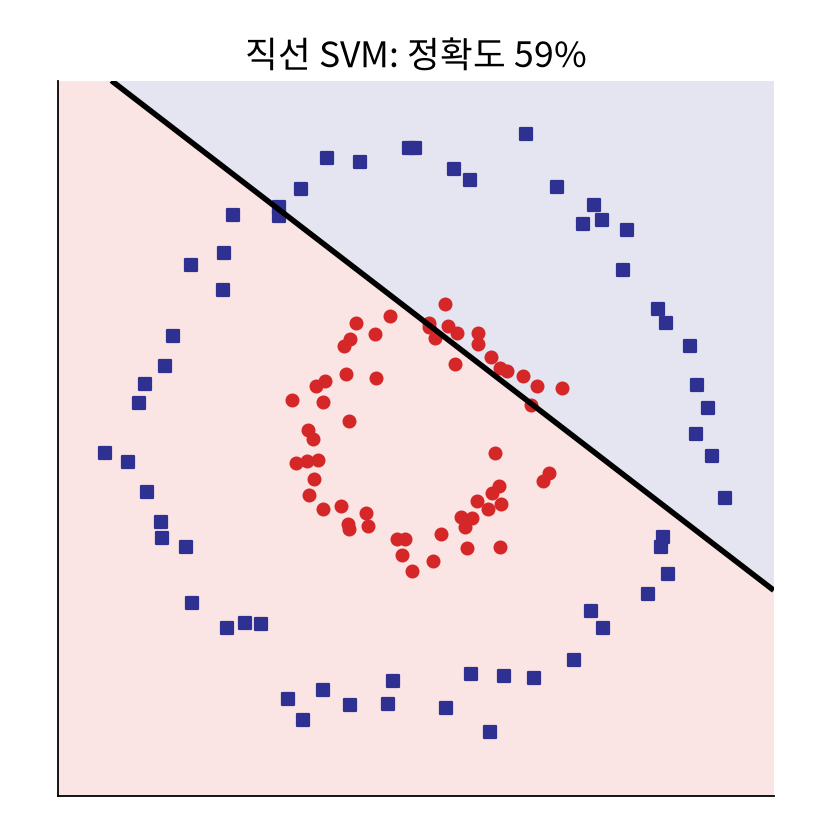
\includegraphics[width=0.95\linewidth]{kn_q.png}\end{column}
\begin{column}{0.52\textwidth}
{\large 빨강이 가운데, 파랑이 바깥 (점 120개)}\\[0.8em]
{\Large \kq{직선 말고 휘어진 경계는\\ 어떻게 만들까?}}
\end{column}
\end{columns}
\vfill
\note{빨간 점이 가운데 모여 있고 파란 점이 바깥을 둘러싼 데이터입니다. 지난 시간의 선형 SVM으로 학습하면 어떤 직선을 그어도 반쯤밖에 못 맞혀서, 정확도가 59퍼센트입니다. 경계가 원이어야 하는데 직선만 그을 수 있기 때문입니다. 오늘은 SVM으로 휘어진 경계를 만드는 방법, 특징 늘리기와 커널을 배웁니다.}
\end{frame}

\section{특징 늘리기}
% --- 1차원 → 2차원
\begin{frame}{가장 쉬운 예: 1차원 점에 $x^2$ 을 붙이면}
\vfill
\centering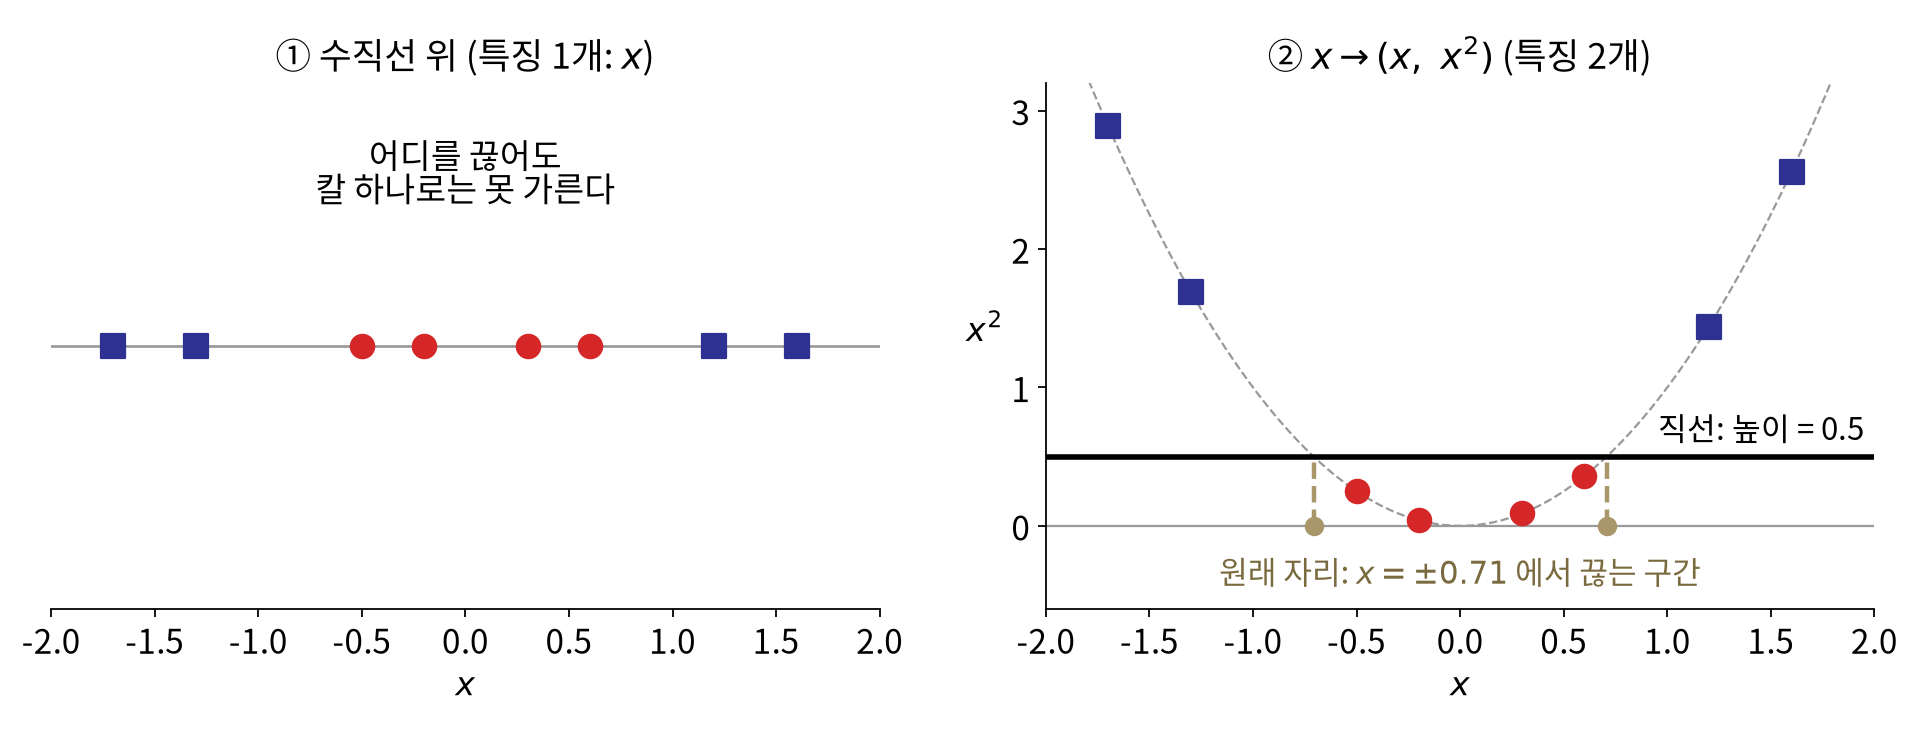
\includegraphics[width=0.9\linewidth]{kn_lift1d.png}\par\vskip0.3em
{\large 특징을 늘리면: 올린 곳에서는 \kb{직선 하나}, 원래 자리에서는 \kq{휘어진 경계} (여기선 구간)}\\[0.2em]
{\normalsize 점마다 $x^2$ 을 계산해서 붙였다 $\to$ \kb{2차원 점}}
\vfill
\note{특징 늘리기를 가장 쉬운 1차원에서 봅시다. 왼쪽은 수직선 위의 점입니다. 빨강이 가운데, 파랑이 양쪽에 있어서, 경계점 하나, 칼질 한 번으로는 어디를 끊어도 가를 수 없습니다. 이제 점마다 숫자를 하나 더 붙입니다. x 제곱입니다. 그러면 점 x가 x, x 제곱, 두 숫자가 되어 오른쪽처럼 평면 위, 포물선 위에 올라갑니다. 가운데 빨강은 낮고 양쪽 파랑은 높습니다. 이제 높이 0.5인 직선 하나로 갈라집니다. 이 직선을 원래 수직선으로 내려 보면, x 제곱이 0.5인 곳, x가 플러스 마이너스 0.71인 두 곳에서 끊는 구간이 됩니다. 특징 수는 점 하나를 숫자 몇 개로 나타내느냐입니다. 1개였던 특징을 2개로 늘리니, 늘린 공간에서는 직선이고 원래 자리에서는 휘어진 경계가 됐습니다. 다음 쪽은 2차원 점에 숫자를 하나 더 붙여 3차원으로 올리는 같은 이야기입니다.}
\end{frame}

% --- 원 모양 데이터
\begin{frame}{특징 늘리기: 직선으로 못 가르면 높이를 준다}
\markpage{lift}
\vfill
\centering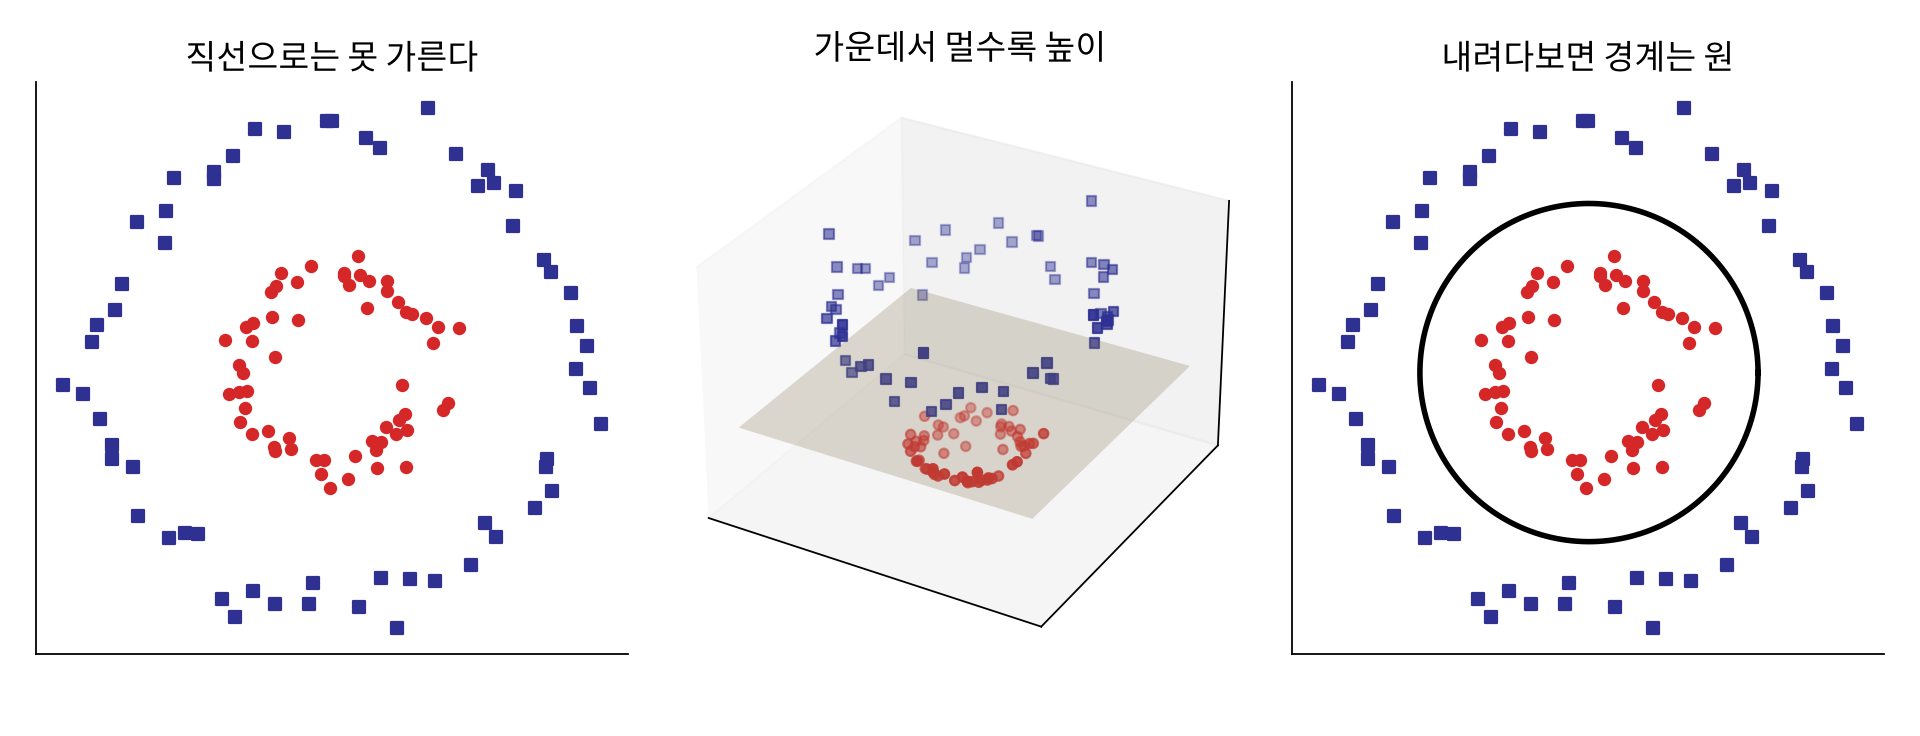
\includegraphics[width=0.8\linewidth]{sv_lift.png}\par\vskip0.2em
{\large $(x_1,\ x_2) \;\to\; (x_1,\ x_2,\ \textcolor{ksablue}{x_1^2 + x_2^2})$}\\[0.2em]{\normalsize 점마다 높이 $x_1^2 + x_2^2$ 를 계산해서 붙였다 $\to$ \kb{3차원 점}}\\[0.2em]
{\normalsize 이렇게 옮기는 것 $= \varphi(\mathbf{x})$, \;옮긴 공간 $=$ \kb{$\varphi$-space} (특징 공간, feature space)}
\vfill
\note{이번에는 빨간 점이 가운데, 파란 점이 바깥을 둘러싼 데이터입니다. 어떤 직선을 그어도 가를 수 없습니다. 그런데 각 점에 높이를 하나 더 줘 봅시다. 가운데서 떨어진 거리의 제곱, x1 제곱 더하기 x2 제곱입니다. 그러면 가운데 빨간 점은 낮게, 바깥 파란 점은 높게 떠서, 가운데 그림처럼 수평한 평면 하나로 깔끔하게 갈라집니다. 이 평면을 원래 평면에서 내려다보면 오른쪽처럼 원이 됩니다. 높은 차원에서 직선으로 가르면, 원래 차원에서는 휘어진 경계가 됩니다. 선형회귀에 x 제곱 특징을 넣은 것과 같은 아이디어입니다. 주의할 점은, 여기서는 세 번째 숫자를 우리가 점마다 실제로 계산해서 붙였다는 것입니다. 정말로 3차원 점을 만든 것이고, 이것은 커널이 아니라 특징을 직접 만든 것입니다. 뒤에서 볼 커널은 이런 숫자를 하나도 만들지 않습니다. 그런데도 결과로 나오는 경계가, 이렇게 숫자를 만들어 올린 뒤 평면으로 가른 것과 같은 모양이 됩니다. 그래서 커널을 높은 차원으로 올린 것처럼 설명하는 것입니다. 이름을 붙여 둡니다. 점에 새 숫자를 만들어 옮기는 것을 파이 x라고 쓰고, 옮겨 놓은 공간을 파이 공간, phi-space라고 부릅니다. 특징 공간, feature space와 같은 말이고 원 논문이 쓰는 표현입니다. 지난 시간에 점마다 알파를 푸는 방식을 배웠는데, 그 방식이 힘을 발휘하는 곳이 바로 이 공간입니다.}
\end{frame}

\section{커널}
% --- 왜 점마다 α 로 푸나 (직접 vs 쌍대)
\begin{frame}{왜 점마다 $\alpha$ 로 푸나: 쌍대 공간 (dual space)}
\vfill
\centering
{\large $\varphi$-space 의 차원 $N$ 이 아주 크거나 \kq{$\infty$} 면 $\mathbf{w}$ 는 직접 못 구한다}\\[0.8em]
\renewcommand{\arraystretch}{1.5}
{\large\begin{tabular}{r|c|c}
 & \textbf{직접} (direct) & \kb{쌍대 (dual)}\\ \hline
구하는 숫자 & \textbf{특징마다} $w_i$ & \kb{점마다} $\alpha_k$\\
숫자 개수 & $N$ ($\varphi$-space 의 차원) & 점 수 $p$\\
예: 빨강 가운데 데이터 (점 120개) & $w_i$ \textbf{6개} & $\alpha_k$ \textbf{120개} (21개만 $\neq 0$)\\
RBF & \kq{$\infty$ 개} & 그래도 \kb{점 수}만큼
\end{tabular}}\\[0.4em]
{\normalsize 예의 특징 6개 $= 1,\ x_1,\ x_2,\ x_1^2,\ x_1x_2,\ x_2^2$ \;·\; 0 아닌 $\alpha$ 21개 $=$ 서포트 벡터}\\[0.6em]
{\large 답은 \textbf{같은 선} \quad 점은 \textbf{점곱} 안에만 $\to$ 그 자리를 바꾸면?}
\vfill
\note{앞 쪽처럼 선형 SVM은 점마다 알파로 쓸 수 있습니다. 왜 이렇게 쓰는 게 좋은지 이제 말할 수 있습니다. 특징을 늘려 파이 공간으로 옮기면, 직접 방식은 특징마다 w를 하나씩 구해야 합니다. 파이 공간의 차원 N이 아주 크면 어렵고, RBF처럼 무한 개면 불가능합니다. 쌍대 방식은 점마다 알파 하나라서, 특징이 몇 개든 점 수만큼만 구합니다. 그리고 답에서는 서포트 벡터만 알파가 0이 아니라 누가 서포트 벡터인지도 보입니다. 오늘의 질문에서 본 빨강이 가운데인 데이터, 점 120개에 특징 6개, 1, x1, x2, x1 제곱, x1 x2, x2 제곱을 쓰면 직접은 w 6개, 쌍대는 알파 120개이고 그중 0이 아닌 것, 서포트 벡터가 21개였습니다. 이 데이터처럼 특징이 적으면 직접이 더 간단하지만, 특징이 많아질수록 쌍대가 이깁니다. 원 논문도 파이 공간의 차원이 크거나 무한하면 직접 푸는 것은 비실용적이고 서포트 벡터에 대한 정보도 얻지 못한다고 하며 쌍대 공간으로 넘어갑니다. 게다가 앞 쪽에서 본 것처럼 점은 점곱 안에만 나옵니다. 그 점곱 자리를 다른 함수로 바꾸면 어떻게 될까요. 그것이 다음 쪽의 커널입니다.}
\end{frame}

% --- 라그랑주 0: 3D 로 보기 (그림 kn_lagrange3d)
\begin{frame}{제약 조건이 있는 최적화: 조건 곡선 위에서 \textbf{가장 높은 점}}
\vfill
\centering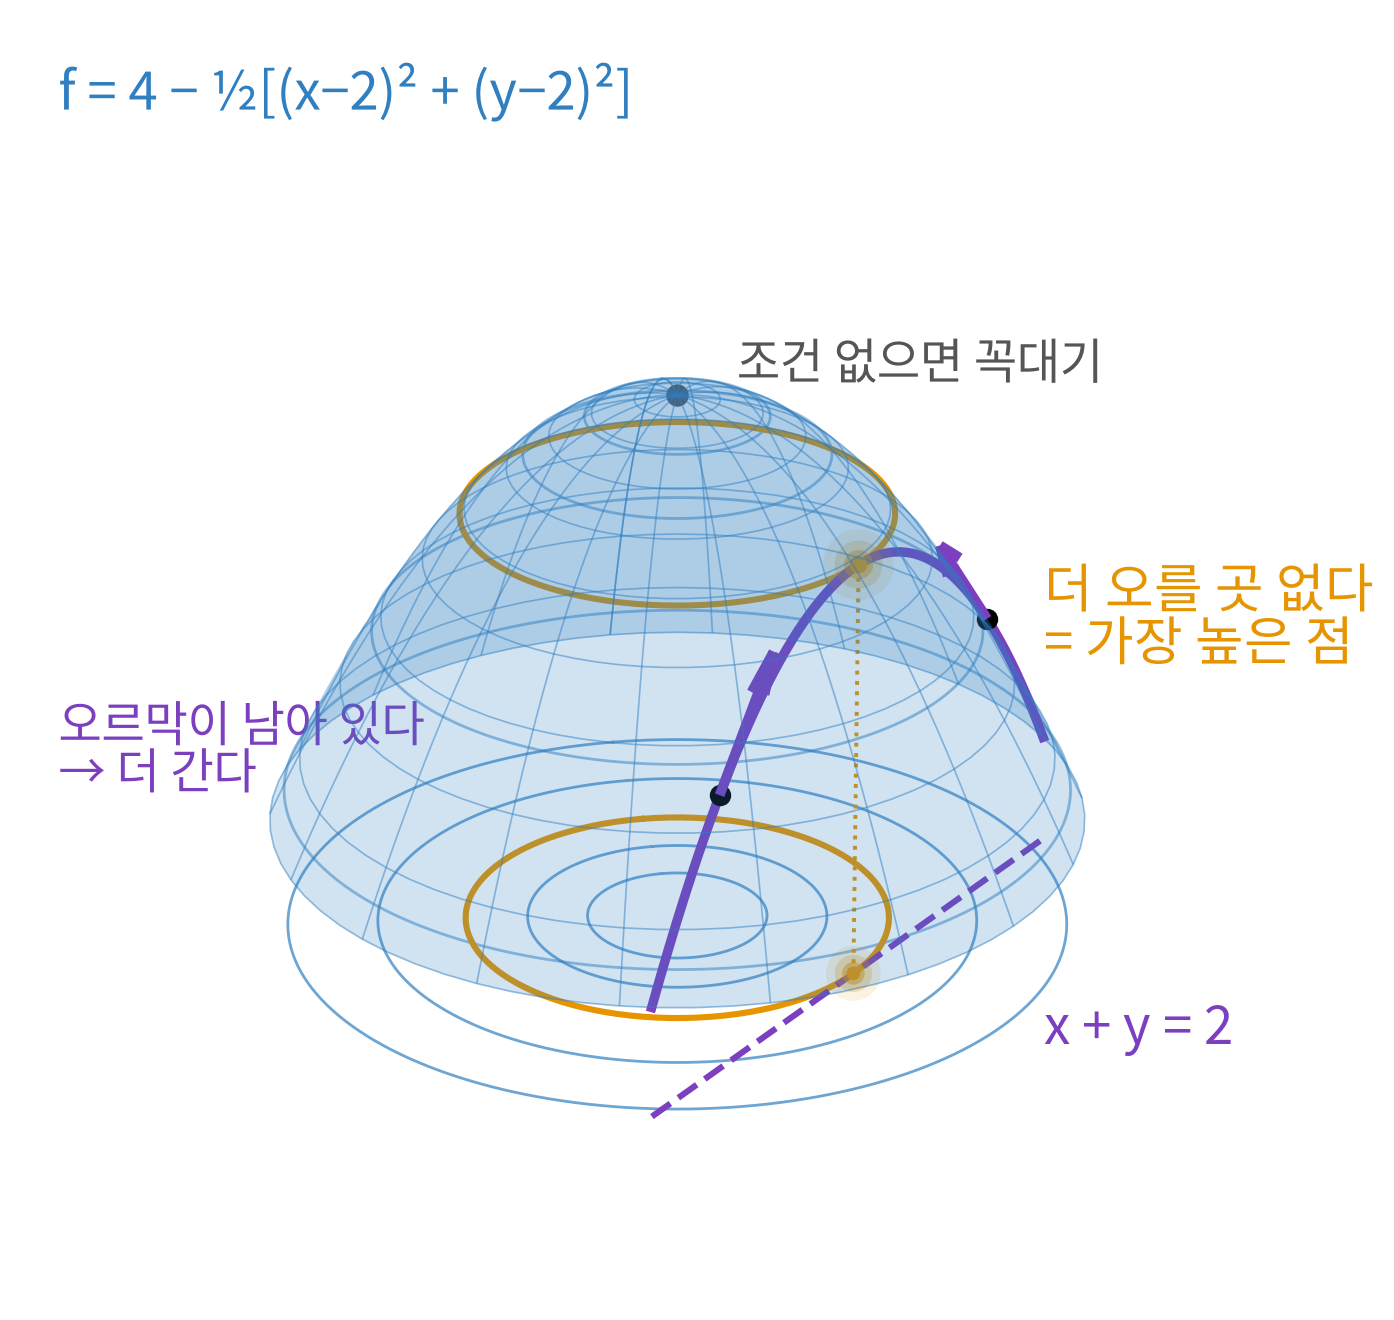
\includegraphics[height=0.70\textheight]{kn_lagrange3d.png}\par\vskip0.2em
{\large $\max\ f = 4 - \tfrac12\big[(x-2)^2 + (y-2)^2\big]$ \quad s.t. \quad $g = x + y - 2 = 0$}\\[0.2em]
{\normalsize 언덕 $= f$ \;·\; 보라 곡선 $=$ 조건을 지키는 점들의 높이 \;·\; 주황 $=$ 그중 가장 높은 점}
\vfill
\note{제약 조건이 있는 최적화를 먼저 그림으로 봅시다. 파란 언덕이 f의 높이이고, 꼭대기는 2, 2에서 높이 4입니다. 조건이 없으면 답은 그냥 꼭대기입니다. 그런데 x 더하기 y가 2여야 한다는 조건이 붙으면, 바닥의 보라 점선 위만 걸을 수 있습니다. 그 점선을 언덕 위로 올리면 보라 곡선, 언덕을 비스듬히 넘어가는 등산로입니다. 이 등산로를 따라 걸으며 가장 높은 곳을 찾는 것이 문제입니다. 주황 점이 그곳이고, 바닥으로 내리면 1, 1, 높이는 3입니다. 바닥의 동심원들은 f가 같은 곳, 등고선이고, 주황 원이 높이 3인 등고선입니다. 이 원이 보라 직선에 딱 맞닿습니다. 가장 낮은 점을 찾는 최소 문제도 언덕을 뒤집은 그릇으로 똑같이 봅니다. SVM이 그 경우입니다. 다음 쪽에서 이 점을 계산으로 찾고, 위에서 내려다본 그림으로 봅니다.}
\end{frame}

% --- 라그랑주 승수법 1: 기본 개념 + 등식 예 (숫자: data.py LG_*)
\begin{frame}{라그랑주 승수법: 조건마다 \textbf{$\alpha$ 를 붙인다}}
\vfill
{\centering\large 제약 조건 $g = 0$ 이 있는 최적화 \;$\to$\; 조건에 \kq{$\alpha$} 를 곱해 목적 함수에서 빼면 \textbf{조건 없는} 문제\par}\vskip0.6em
\begin{columns}[c]
\begin{column}{0.42\textwidth}\centering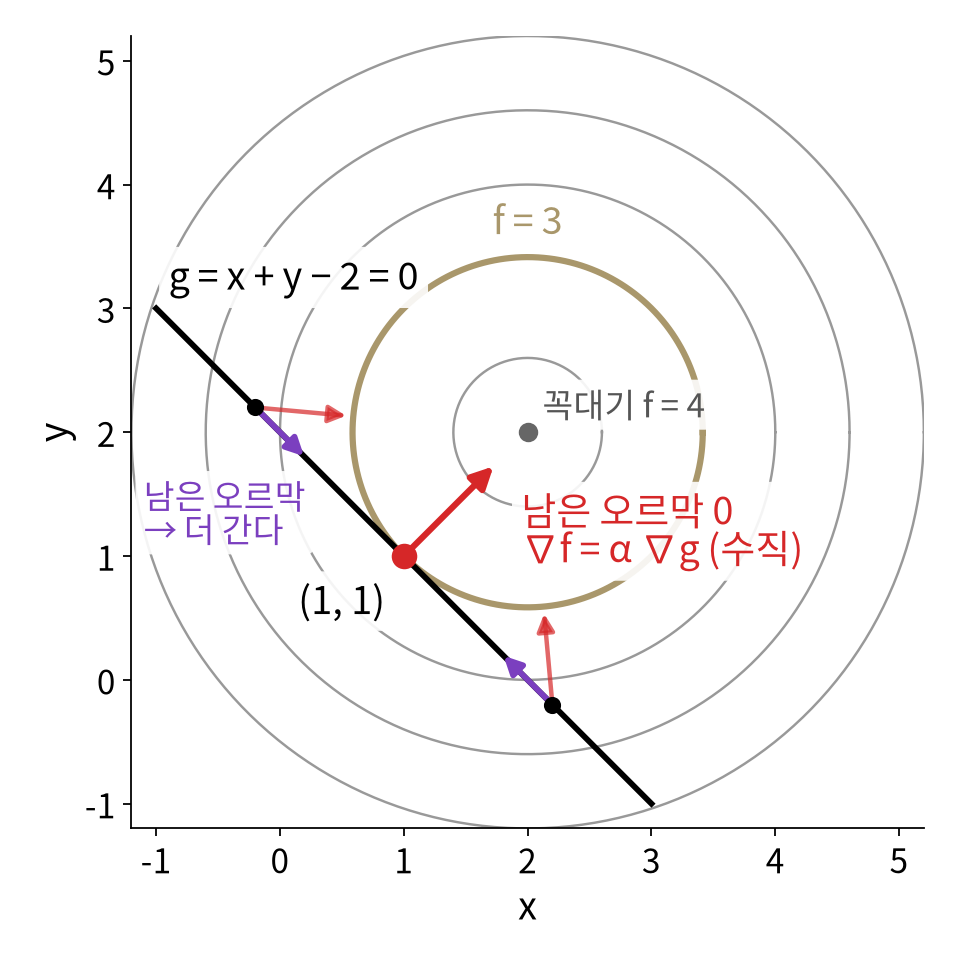
\includegraphics[height=0.60\textheight]{kn_lagrange.png}\end{column}
\begin{column}{0.57\textwidth}
{\large $\max\ f = 4 - \tfrac12\big[(x-2)^2 + (y-2)^2\big]$}\\[0.2em]
{\large s.t. \; $g = x + y - 2 = 0$ \quad {\normalsize (등식 조건)}}\\[0.6em]
{\large $L(x, y, \textcolor{ksared}{\alpha}) = f - \textcolor{ksared}{\alpha}\, g$ \quad {\normalsize (조건 없는 문제로)}}\\[0.6em]
\renewcommand{\arraystretch}{1.3}
{\small\begin{tabular}{l@{\;}l}
$\partial L/\partial x = -(x - 2) - \alpha = 0$ & \\
$\partial L/\partial y = -(y - 2) - \alpha = 0$ & $\to\ x = y = 2 - \alpha$\\
$\partial L/\partial \alpha = -g = 0$ & $\to\ 4 - 2\alpha = 2$\\
 & $\to\ \textcolor{ksared}{\alpha = 1}$, \;$(x, y) = (1, 1)$
\end{tabular}}\\[0.6em]
{\normalsize 답에서 $f$ 등고선과 조건 직선이 \kb{맞닿는다}}\\[0.1em]{\normalsize $\to$ 둘 다 그 점에서 직선에 \textbf{수직}: $\nabla f = \alpha \nabla g$}
\end{column}
\end{columns}
\vfill
\note{SVM은 제약 조건이 있는 최적화 문제입니다. 이런 문제는 조건마다 알파라는 숫자를 하나씩 붙여서 풉니다. 이것이 라그랑주 승수법입니다. 생각은 하나, 조건에 알파를 곱해 목적 함수 안으로 옮겨서 조건 없는 문제로 바꾸는 것입니다. 앞 쪽의 언덕으로 해 봅시다. 4 빼기 2분의 1 곱하기 x 빼기 2의 제곱 더하기 y 빼기 2의 제곱을 가장 크게 하되, x 더하기 y 빼기 2가 0이어야 합니다. 조건 g에 숫자 알파를 곱해 f에서 빼면 라그랑주 함수 L입니다. 이 알파가 라그랑주 승수입니다. 이제 조건을 따로 신경 쓰지 않고, x, y, 알파 세 변수로 각각 편미분해서 모두 0이 되는 곳을 찾습니다. x로 미분하면 마이너스 x 빼기 2, 빼기 알파이고, y도 같은 꼴이라 x와 y는 둘 다 2 빼기 알파입니다. 알파로 미분하면 마이너스 g, 즉 조건 그 자체가 나오니 4 빼기 2알파가 2, 알파는 1이고 답은 1, 1입니다. 그림은 앞의 언덕을 위에서 내려다본 것입니다. 회색 동심원이 f가 같은 곳, 등고선이고 가운데 점이 꼭대기, 검은 직선이 조건입니다. 직선 위를 따라가며 f가 가장 큰 곳은 금색 원, 높이 3인 등고선이 직선에 딱 맞닿는 곳입니다. 맞닿는다는 것은 그 점에서 두 선의 수직 방향이 같다는 뜻입니다. 빨간 화살표가 f의 기울기, 오르막 방향으로 꼭대기를 향합니다. 1, 1이고, 직선 x 더하기 y가 2에 정확히 수직입니다. g의 기울기도 1, 1이라 둘이 같은 방향이고, 그 비율이 알파, 1입니다. 아직 오르막이 직선을 따라 남아 있다면 더 걸어 올라갈 수 있으니, 가장 높은 점에서는 오르막이 직선에 수직일 수밖에 없습니다. 편미분이 0이라는 식이 바로 이 조건입니다.}
\end{frame}

% --- 라그랑주 승수법 1-9: 지난 시간 식 (‖w‖=1, max M) → min ½‖w‖² (크기 맞추기)
\begin{frame}{지난 시간 식을 바꿔 쓰기: 최대 $M$ $\to$ 최소 $\tfrac12\lVert\mathbf{w}\rVert^2$}
\vfill
\centering
\renewcommand{\arraystretch}{1.5}
{\large\begin{tabular}{c|c}
지난 시간 & 오늘\\ \hline
$\max\ M$ & $\min\ \tfrac12\lVert\mathbf{w}\rVert^2$\\
크기 약속: $\lVert\mathbf{w}\rVert = 1$ & 크기 약속: \kb{$M\lVert\mathbf{w}\rVert = 1$}\\
$y_k(\mathbf{w}\cdot\mathbf{x}_k + b) \ge M$ & $y_k(\mathbf{w}\cdot\mathbf{x}_k + b) \ge 1$\\ \hline
\small $\mathbf{w} = (0.71, 0.71)$, $b = 0.035$, $M = 0.67$ & \small $\mathbf{w} = (1.05, 1.05)$, $b = 0.053$, $\lVert\mathbf{w}\rVert = 1.49$
\end{tabular}}\\[1.0em]
{\normalsize $\mathbf{w}, b$ 를 \kb{$1/M$ 배} \;$\to$\; 가장 가까운 점이 $M \to 1$, \;길이 $1 \to 1/M$ \quad ($0.71/0.67 = 1.05$)}\\[0.3em]
{\normalsize 그래서 $M = 1/\lVert\mathbf{w}\rVert$ \;$\to$\; \kb{$M$ 최대 $=$ $\lVert\mathbf{w}\rVert$ 최소} \;$=$\; $\tfrac12\lVert\mathbf{w}\rVert^2$ 최소}\\[0.3em]
{\small $\tfrac12$ 과 제곱: 답은 같고 미분이 깔끔 ($\nabla \tfrac12\lVert\mathbf{w}\rVert^2 = \mathbf{w}$)}
\vfill
\note{지난 시간 끝에 쓴 최대 마진 식을 라그랑주 승수법에 맞는 꼴로 바꿉니다. 지난 시간에는 w의 길이를 1로 맞추고, 모든 점이 경계에서 M 이상 떨어지도록 하면서 M을 최대로 했습니다. 이 데이터의 답은 w가 0.71, 0.71, b가 0.035, M이 0.67이었습니다. 이제 w와 b를 함께 M분의 1배, 즉 0.67로 나눕니다. 경계 직선은 식 전체에 같은 수를 곱해도 그대로이니 분류기는 바뀌지 않습니다. 대신 가장 가까운 점의 값 y k D x k가 M에서 1이 되고, w의 길이는 1에서 M분의 1, 1.49가 됩니다. w는 0.71 나누기 0.67, 1.05, 1.05가 되고, b는 0.035 나누기 0.67, 0.053이 됩니다. 그러면 마진 M은 1 나누기 w의 길이이고, M을 가장 크게 하는 것은 w의 길이를 가장 작게 하는 것과 같습니다. 크기 약속이 w의 길이가 1에서 M 곱하기 w의 길이가 1로 바뀐 것입니다. 이 약속은 w로 M이 정해진다는 뜻이라 따로 풀 조건이 아니고, 남는 조건은 모든 점이 1 이상이라는 것뿐입니다. 길이를 최소로 하는 대신 2분의 1 길이 제곱을 최소로 해도 답은 같은데, 미분하면 w 자신이 나와서 계산이 깔끔합니다. 이제부터는 이 오른쪽 식을 씁니다. 알파 값도 이 약속에서 구한 것이라 첫 쪽의 알파와 크기가 다르고 비율만 같습니다.}
\end{frame}

% --- 라그랑주 승수법 2-00: 원통을 키우다 처음 닿는 곳 = 답 (그림 kn_lagrange_svm_grow)
\begin{frame}{SVM 을 $(w_1, w_2, b)$ 공간에서: 원통을 \textbf{키우다 처음 닿는 곳}}
\vfill
\centering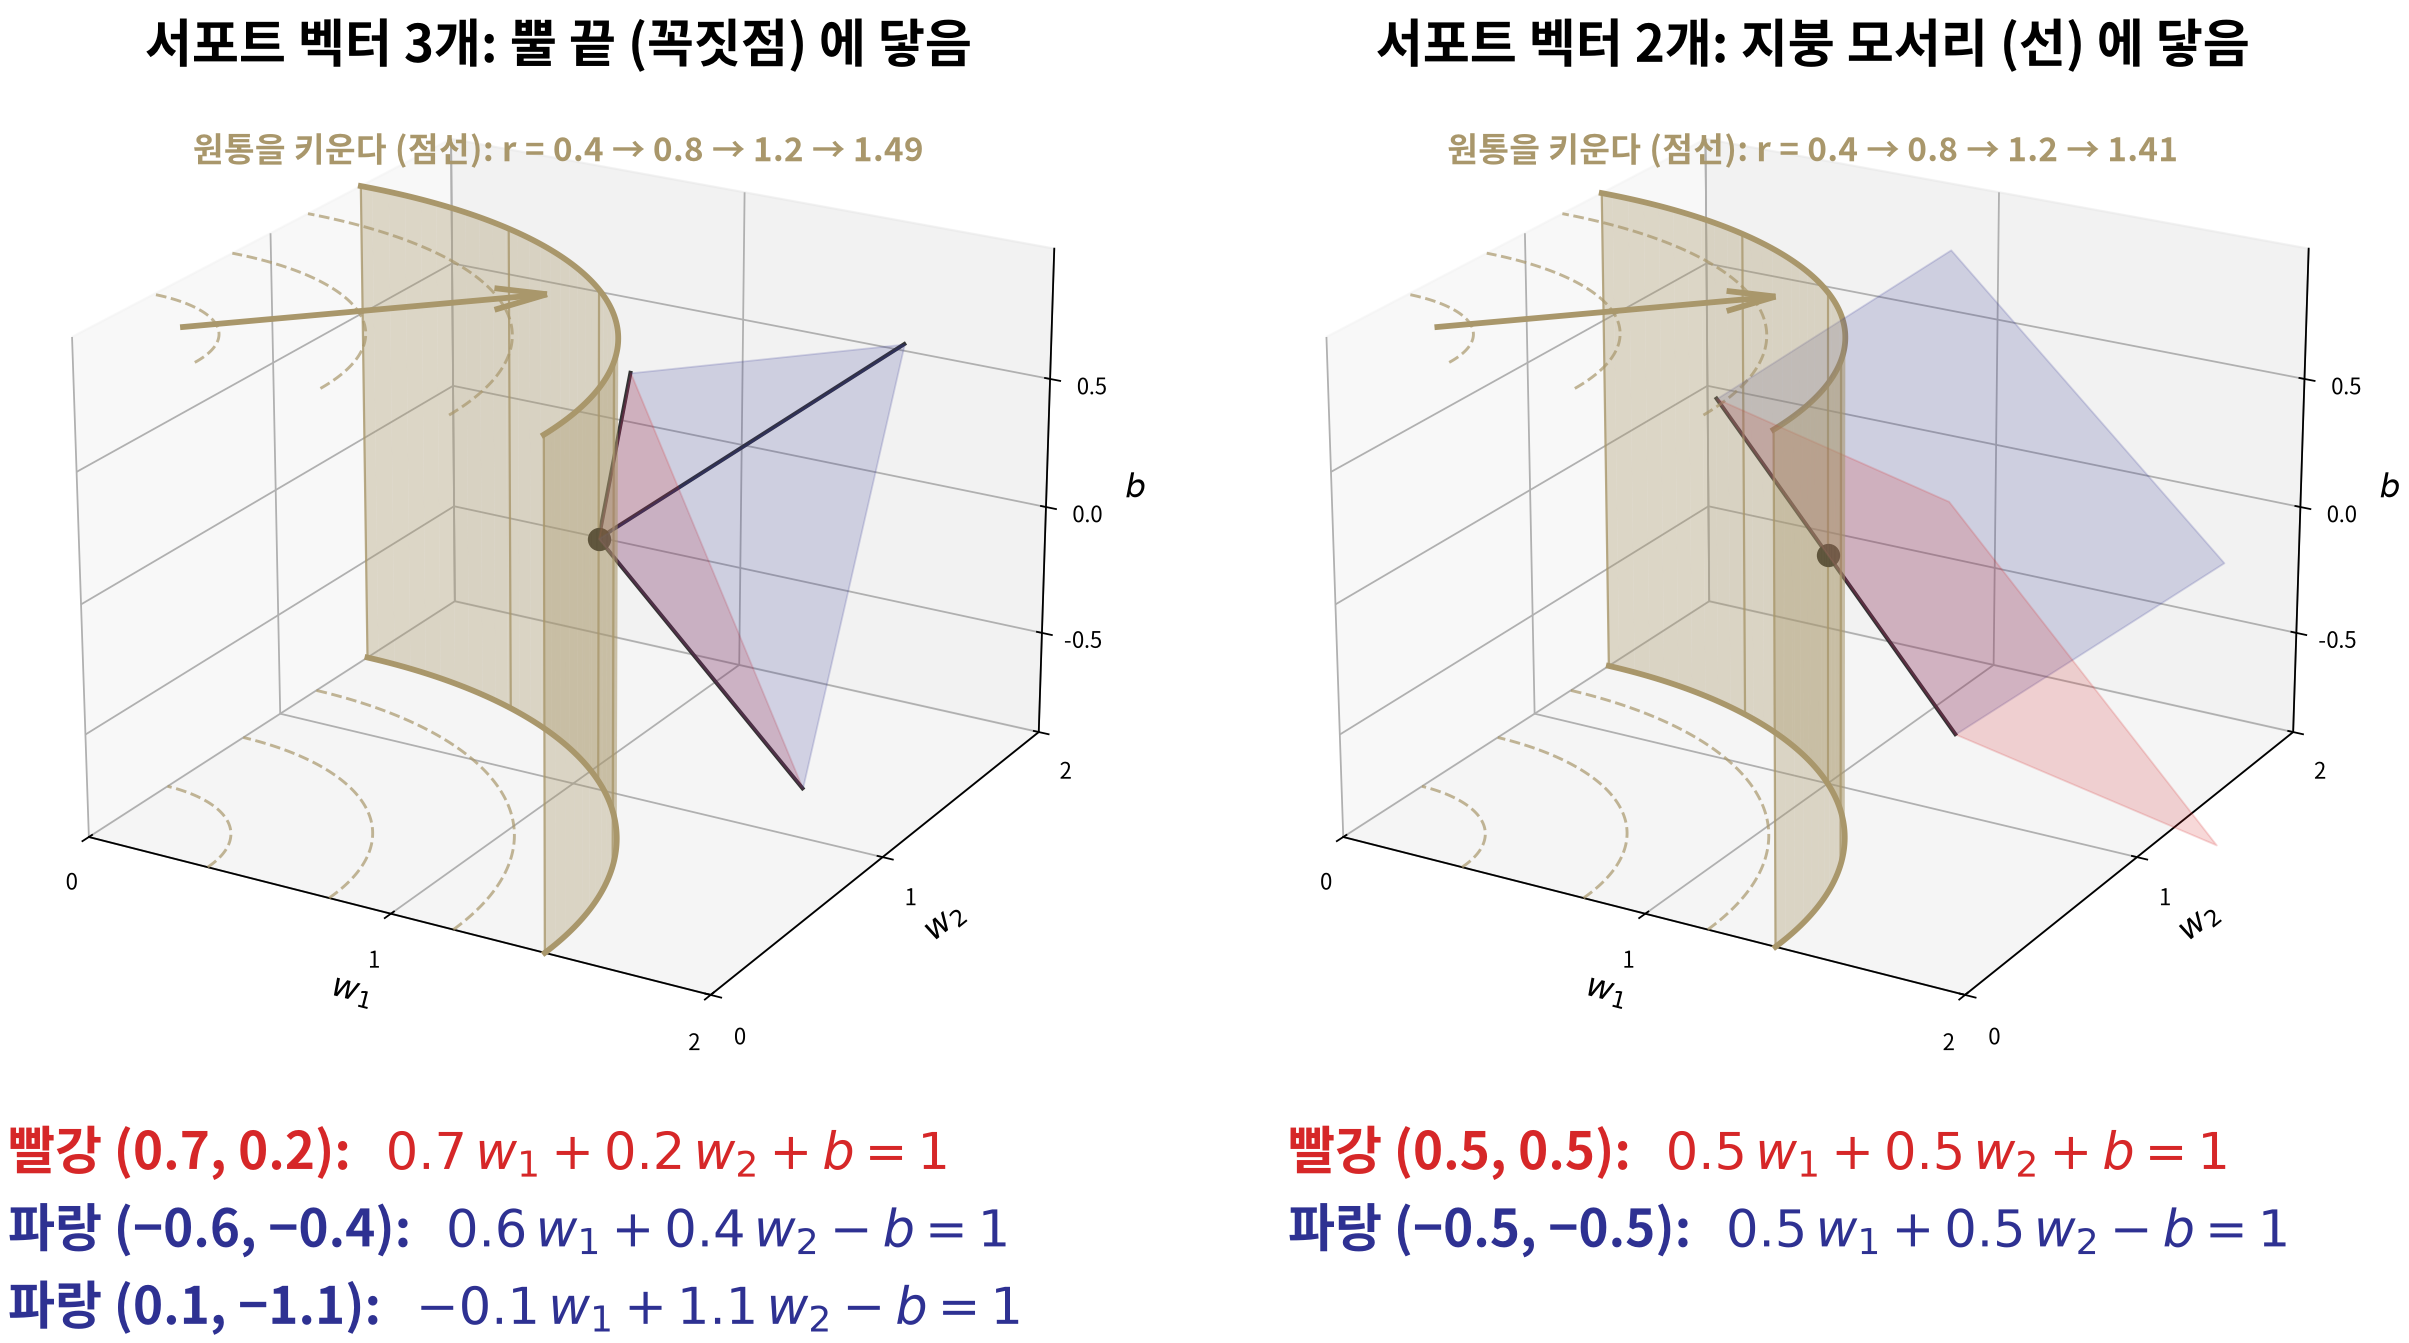
\includegraphics[height=0.70\textheight]{kn_lagrange_svm_grow.png}\par\vskip0.1em
{\small \textcolor{fbeta}{원통} $=$ $\tfrac12\lVert\mathbf{w}\rVert^2$ 가 같은 곳 \;·\; 평면이 깎은 곳 $=$ 조건을 다 지키는 곳 \;·\; 처음 닿는 점 $= (\mathbf{w}^*, b^*)$}\\[0.05em]
{\small 무작위 2차원 데이터 2,000번: 서포트 벡터 \kb{2개 46\%} · \kb{3개 54\%} · 4개 0.2\% (점이 한 직선에 놓인 우연)}
\note{SVM을 언덕 예처럼 그림으로 봅시다. 그림 아래의 식이 서포트 벡터마다의 평면 식입니다. 예를 들어 빨간 점 0.7, 0.2는 y가 1이라 0.7 w1 더하기 0.2 w2 더하기 b가 1이고, 파란 점 마이너스 0.6, 마이너스 0.4는 y가 마이너스 1이라 부호가 바뀌어 0.6 w1 더하기 0.4 w2 빼기 b가 1입니다. 왼쪽은 우리 점 20개입니다. SVM이 구하는 숫자는 w1, w2, b 세 개라서 3차원 공간에서 봅니다. 점 하나의 조건, y k 곱하기 w 점곱 x k 더하기 b가 1 이상이라는 식은 이 공간에서 평면 한 장의 한쪽입니다. 서포트 벡터 세 점의 평면, 빨강 하나와 파랑 둘이 깎아 낸 뿔 모양이 조건을 다 지키는 곳입니다. 그 뿔의 끝, 뾰족한 모서리가 답 근처의 모양입니다. 금색 원통은 2분의 1 w 길이 제곱이 같은 곳입니다. b가 들어 있지 않아서 b 방향으로 쭉 뻗은 원통입니다. 우리가 원하는 것은 w의 길이가 가장 작은 것, 즉 원통이 가장 가는 것입니다. 그러니 원통 반지름을 0부터 조금씩 키워 봅니다. 점선이 키우는 중의 원통입니다. 0.4, 0.8, 1.2일 때는 뿔에 닿지 않습니다. 조건을 지키는 w가 그 원통 안에는 하나도 없다는 뜻입니다. 1.49가 되는 순간 뿔의 끝에 처음 닿습니다. 그 점이 답, w 별과 b 별이고, 마진은 1 나누기 1.49, 0.67입니다. 언덕 예에서 등산로를 따라 더 오를 곳이 없는 점을 찾았듯이, 여기서는 원통을 키우다 처음 닿는 점을 찾습니다. 원통이 뿔 끝, 평면 세 장이 만나는 꼭짓점에 닿았으니 서포트 벡터가 세 개입니다. 오른쪽은 지난 시간의 작은 예, 점 8개입니다. 서포트 벡터가 빨강 0.5, 0.5와 파랑 마이너스 0.5, 마이너스 0.5 두 개뿐입니다. 평면이 두 장이라 뿔 대신 지붕 모양이고, 지붕의 모서리는 점이 아니라 선, b가 0이고 w1 더하기 w2가 2인 직선입니다. 언덕 예의 조건 직선 x 더하기 y가 2와 같은 직선입니다. 원통을 키우면 1.41에서 이 모서리 선에 옆으로 맞닿고, 그 점 1, 1, 0이 답입니다. 언덕 예에서 등고선이 직선에 맞닿았던 것과 똑같은 모양입니다. 어느 쪽이 흔할까요. 겹치지 않는 2차원 점 20개를 무작위로 2천 번 만들어 세어 보니, 서포트 벡터 2개가 46퍼센트, 3개가 54퍼센트로 둘 다 흔합니다. 4개는 0.2퍼센트, 점들이 우연히 한 직선 위에 놓인 경우뿐입니다. 3차원 공간에서 평면 세 장이 한 점에서 만나는 것은 당연하지만, 네 장이 만나는 것은 우연이기 때문입니다.}
\end{frame}

% --- 라그랑주 승수법 2-0: (w1, w2, b) 3D 에서 조건 = 평면, 답 = 모서리, b = b* 로 자르기 (그림 kn_lagrange_svm3d)
\begin{frame}{SVM 을 $(w_1, w_2, b)$ 공간에서: 조건 하나 $=$ \textbf{평면} 하나}
\vfill
\begin{columns}[c]
\begin{column}{0.47\textwidth}\centering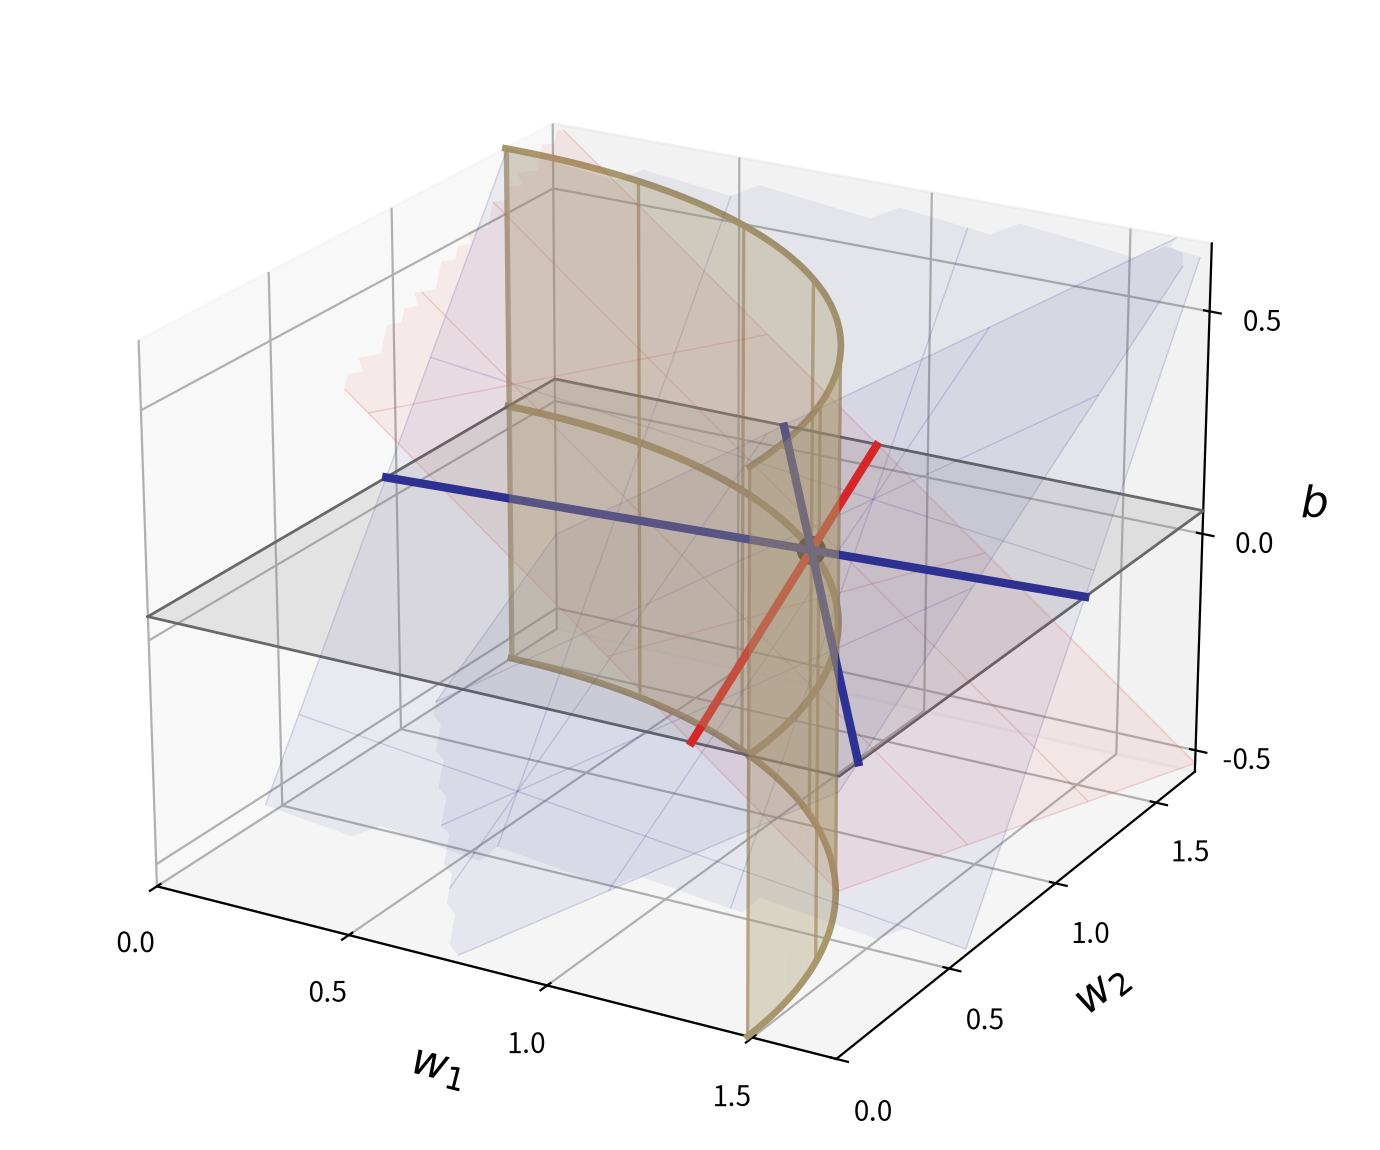
\includegraphics[width=\linewidth]{kn_lagrange_svm3d.png}\end{column}
\begin{column}{0.52\textwidth}
{\normalsize 축 3개 $= w_1,\ w_2,\ b$ ($b$ 도 축 \;$\to$ 몰라도 그린다)}\\[0.25em]
{\normalsize 점 $\mathbf{x}_k$ 하나 $=$ \textbf{평면} 하나 ($\mathbf{x}_k, y_k$ 는 숫자)}\\[0.1em]
{\small 예: \textcolor{ksared}{빨강} $(0.7, 0.2)$ $\to$ $0.7w_1 + 0.2w_2 + b = 1$}\\[0.25em]
{\normalsize 검은 점 $=$ 세 면의 \textbf{모서리} $(\mathbf{w}^*, b^*)$}\\[0.25em]
{\normalsize \textcolor{fbeta}{금색} $=$ $\tfrac12\lVert\mathbf{w}\rVert^2$ 등고선 (원기둥)}\\[0.25em]
{\normalsize 회색 $=$ \kb{$b = b^*$ 로 자른 면} $\to$ 직선 3개 $+$ 원}\\[0.6em]
\renewcommand{\arraystretch}{1.15}
{\footnotesize\begin{tabular}{@{}l|c|c@{}}
 & 데이터 $(x_1, x_2)$ & $(w_1, w_2, b)$\\ \hline
점 $\mathbf{x}_k$ & 점 & 평면\\
분류기 $(\mathbf{w}, b)$ & 직선 & 점
\end{tabular}}
\end{column}
\end{columns}
\vfill
\note{여기서는 무엇이 변수인지가 지난 시간과 뒤바뀝니다. 지난 시간 그림은 w와 b를 정해 두고 x를 움직여서, 데이터 점은 점이고 분류기는 직선이었습니다. 이 그림은 데이터 점 x k와 y k가 정해진 숫자이고 w1, w2, b가 움직입니다. 그래서 분류기 하나가 이 공간의 점 하나이고, 데이터 점 하나는 평면 하나입니다. 예를 들어 빨간 서포트 벡터 0.7, 0.2의 조건은 0.7 w1 더하기 0.2 w2 더하기 b가 1이라는 식이고, 미지수 세 개의 일차식이라 평면입니다. b도 축 하나라서 b를 몰라도 이 평면을 그릴 수 있습니다. b를 알아야 하는 것은 b 별로 자른 단면을 그릴 때뿐입니다. 다음 쪽 그림에서 세 직선이 한 점에서 만나는 것이 우연처럼 보일 수 있습니다. 평면에 직선 세 개를 아무렇게나 그으면 한 점에서 만나는 일은 거의 없으니까요. 그런데 SVM이 구하는 숫자는 w1, w2, b 세 개입니다. 그러니 진짜 공간은 3차원이고, 점 하나의 조건, y k 곱하기 w 점곱 x k 더하기 b가 1이라는 식은 이 공간에서 평면 한 장입니다. 그림의 빨간 면 하나와 파란 면 둘이 서포트 벡터 세 점의 조건입니다. 3차원에서 평면 세 장은 방의 모서리처럼 한 점에서 만나는 것이 자연스럽고, 그 모서리가 답, w 별과 b 별입니다. 금색은 2분의 1 w 길이 제곱이 같은 곳인데, b가 들어 있지 않아서 b 방향으로 쭉 뻗은 원기둥입니다. 이제 이 공간을 b가 b 별인 회색 수평면으로 자릅니다. 그러면 세 평면은 굵은 직선 세 개로, 원기둥은 금색 원으로 잘립니다. 다음 쪽의 그림이 바로 이 회색 단면입니다. 모서리를 지나도록 잘랐으니 세 직선이 한 점에서 만나는 것은 당연합니다. b를 다른 값으로 잘랐다면 세 직선은 보통 한 점에서 만나지 않습니다. 서포트 벡터가 두 개일 때는 평면 두 장만 답을 지나고, 두 평면이 만나는 선 위에서 원기둥이 그 선에 옆으로 맞닿는 곳이 답입니다. 이때도 b가 b 별인 단면에서는 직선 두 개가 w 별에서 만납니다. 원이 직선에 옆으로 맞닿는 모양은 단면이 아니라, b 축을 따라 위에서 내려다볼 때 보입니다.}
\end{frame}

% --- 라그랑주 승수법 2: SVM 의 L 을 w 평면에서 (그림 kn_lagrange_svm)
\begin{frame}{SVM 도 제약 조건이 있는 최적화: 점마다 $\alpha_k$}
\vfill
\centering
{\large $\min\ \tfrac12\lVert\mathbf{w}\rVert^2$ \;\; s.t. \;\; $y_k(\mathbf{w}\cdot\mathbf{x}_k + b) - 1 \ge 0$ \qquad $L = \tfrac12\lVert\mathbf{w}\rVert^2 - \sum_{k=1}^{p} \textcolor{ksared}{\alpha_k}\,\big[\,y_k(\mathbf{w}\cdot\mathbf{x}_k + b) - 1\,\big]$}\\[0.2em]
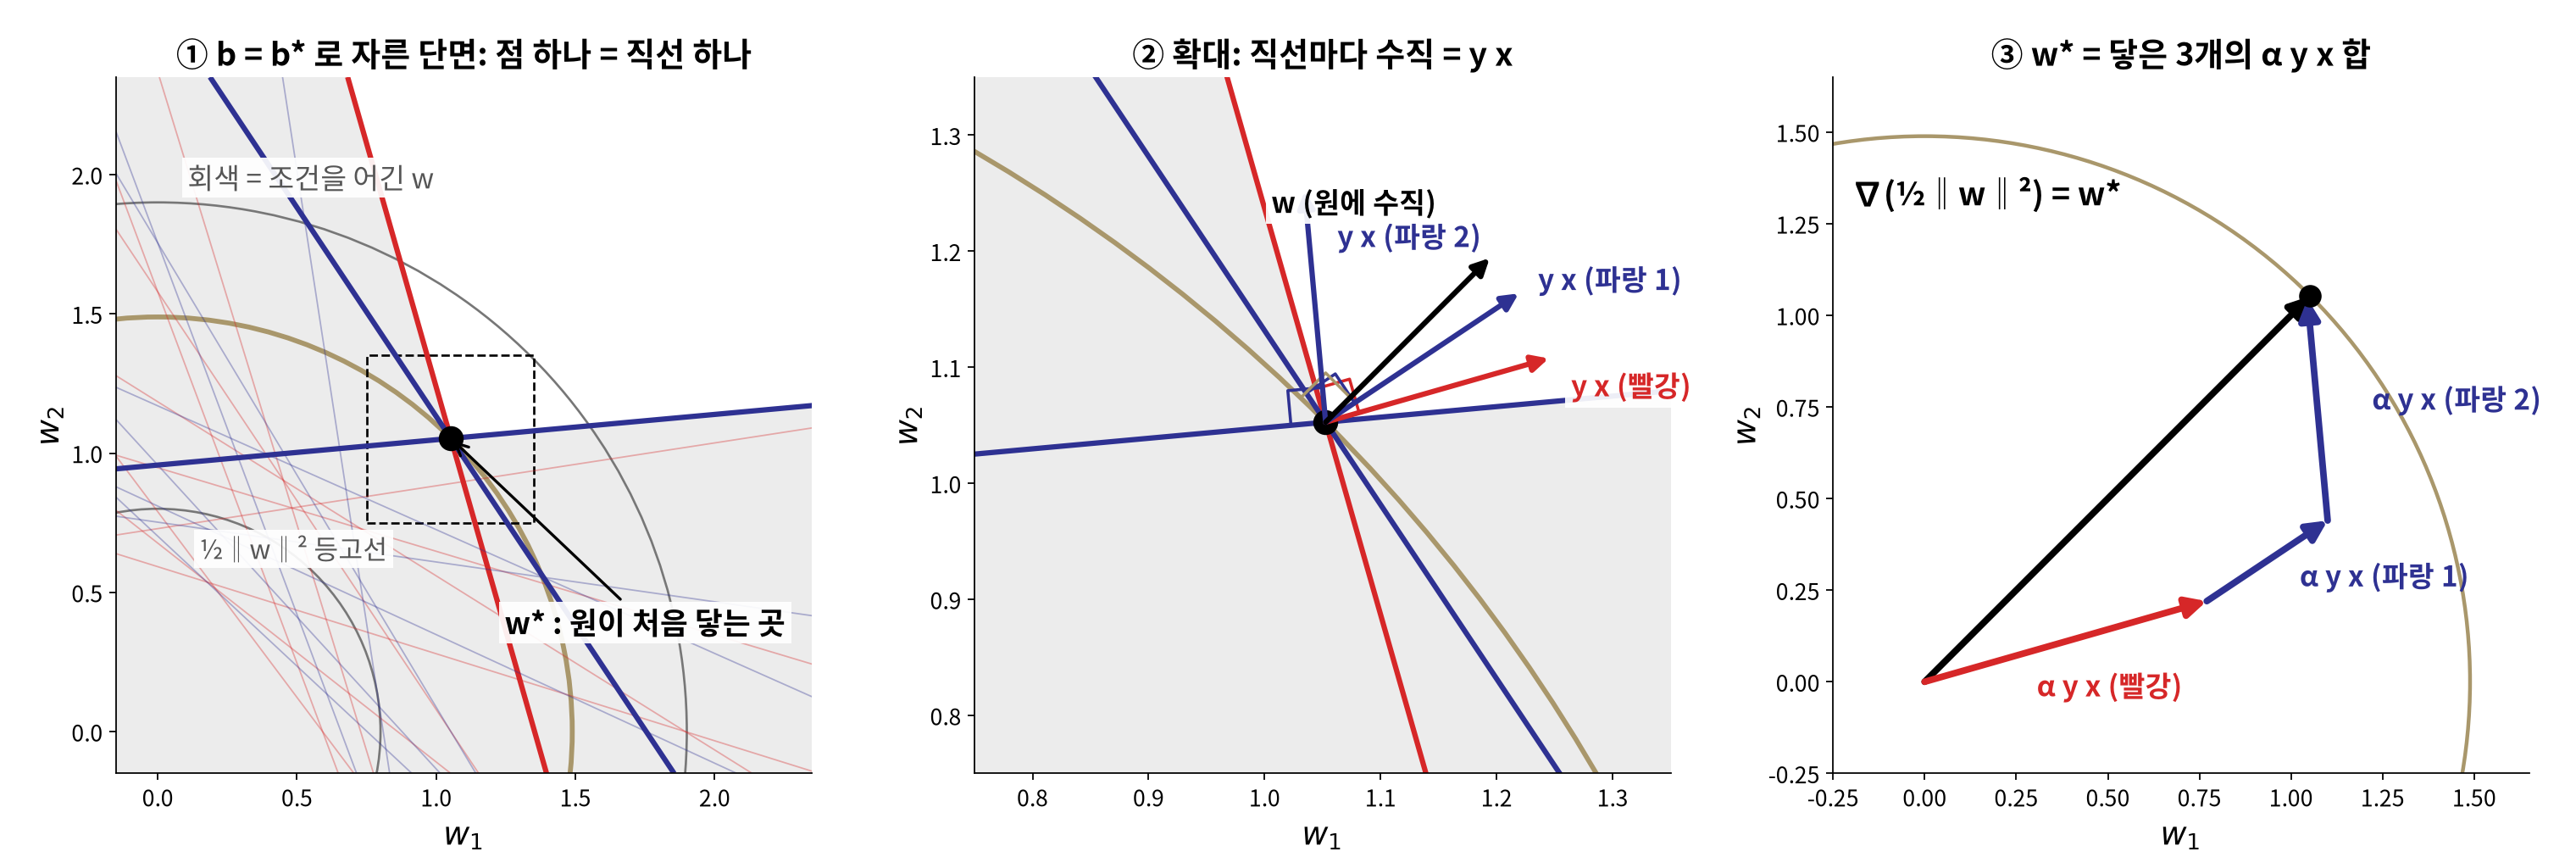
\includegraphics[height=0.42\textheight]{kn_lagrange_svm.png}\par\vskip0.1em
{\normalsize 답에서 $\nabla\big(\tfrac12\lVert\mathbf{w}\rVert^2\big) = \sum_k \alpha_k \nabla g_k$ \;$\to$\; \kb{$\mathbf{w} = \sum_k \alpha_k y_k \mathbf{x}_k$} \quad (앞 예의 $\nabla f = \alpha\nabla g$)}\\[0.1em]
{\small $g_k = y_k(\mathbf{w}\cdot\mathbf{x}_k + b) - 1$: 점 $k$ 의 조건 (직선 하나) \;$\to$\; $\mathbf{w}$ 로 미분하면 $\nabla g_k = y_k\mathbf{x}_k$}\\[0.1em]
{\small 서포트 벡터 3개: $w_1, w_2$ 두 식 $+$ $b$ 로 미분한 $\sum_k \alpha_k y_k = 0$ \;$\to$\; \kb{식 3개 · 미지수 $\alpha$ 3개}}
\vfill
\note{SVM도 제약 조건이 있는 최적화 문제라서, 똑같이 조건마다 알파를 붙입니다. 앞에서 바꿔 쓴 대로 문제는 2분의 1 w 길이 제곱을 최소로 하되 모든 점이 y k 곱하기 w 점곱 x k 더하기 b, 빼기 1이 0 이상이어야 한다입니다. 조건이 점마다 하나씩이니 승수도 점마다 알파 k 하나씩 붙여 빼면 L입니다. 그림은 이 문제를 w 평면에서 본 것입니다. 가로축 w1, 세로축 w2이고, b는 답의 값으로 고정했습니다. 앞 예에서 조건이 직선 하나였듯이, 여기서는 점 하나가 조건 하나, 직선 하나입니다. 20개 점이니 직선이 20개이고, 그중 하나라도 어기는 w는 회색입니다. 금색 원은 2분의 1 w 길이 제곱이 같은 곳, 등고선입니다. 원을 점점 키우다 흰 곳에 처음 닿는 점이 답 w 별입니다. 앞 예에서 등고선이 직선에 맞닿았던 것과 같습니다. 다만 여기서는 직선 세 개가 만나는 모서리에 닿습니다. 굵은 빨강 하나, 파랑 둘이 그 세 점, 서포트 벡터입니다. 오른쪽 그림이 그 점에서의 기울기입니다. 2분의 1 w 길이 제곱의 기울기는 w 자신이고, 조건 g k, 즉 점 k의 y k 곱하기 w 점곱 x k 더하기 b, 빼기 1을 w로 미분한 기울기는 y k x k입니다. 앞 예의 기울기 f는 알파 곱하기 기울기 g가, 조건이 여러 개라 알파 k 곱하기 기울기 g k의 합이 됩니다. 그래서 w 별은 닿은 세 점의 알파 y x를 더한 것입니다. 그런데 이 합이 w 별과 딱 같아지는 것은 우연이 아니라, 알파를 그렇게 되도록 정한 것입니다. 서포트 벡터가 세 개면 알파도 세 개입니다. 식은 w 별의 w1 성분과 w2 성분이 맞아야 한다는 두 개, 그리고 L을 b로 미분해서 나오는 알파 k y k의 합이 0이라는 하나, 모두 세 개입니다. 식 세 개에 미지수 세 개라 알파가 한 번에 정해집니다. 진짜 조건은 이렇게 구한 알파가 모두 0 이상이냐는 것이고, 원통이 처음 닿는 점에서만 그렇습니다. 이 쪽은 가장 가까운 값을 1로 맞춘 약속이라 알파의 크기는 첫 쪽과 다르고, 비율만 같습니다.}
\end{frame}

% --- 라그랑주 승수법 3: 부등식이라 규칙 둘 더 = KKT
\begin{frame}{조건이 \textbf{$\ge$} 라서 규칙 둘 더: KKT 조건}
\vfill
\centering
{\Large $L(\mathbf{w}, b, \textcolor{ksared}{\alpha}) = \tfrac12\lVert\mathbf{w}\rVert^2 - \sum_{k=1}^{p} \textcolor{ksared}{\alpha_k}\,\big[\,y_k(\mathbf{w}\cdot\mathbf{x}_k + b) - 1\,\big]$}\\[0.8em]
\renewcommand{\arraystretch}{1.5}
{\large\begin{tabular}{rl}
\textbf{1.} & $\partial L/\partial\mathbf{w} = 0$, \quad $\partial L/\partial b = 0$\\
\textbf{2.} & $\alpha_k \ge 0$ \quad {\normalsize (못은 밀기만 한다)}\\
\textbf{3.} & $\alpha_k = 0$ \;또는\; $y_k(\mathbf{w}\cdot\mathbf{x}_k + b) = 1$ \quad {\normalsize $\to$ 길 가장자리 점 (\kb{서포트 벡터}) 만 $\alpha_k \neq 0$}
\end{tabular}}\\[0.6em]
{\normalsize 앞의 예는 $= 0$ 이라 1 만, \;SVM 은 $\ge 0$ (안 닿는 점이 있다) 이라 2 · 3 이 더 붙는다 \;$=$ \textbf{KKT 조건}}\\[0.1em]
{\small KKT = Karush (1939) · Kuhn · Tucker (1951)}
\vfill
\note{앞의 예와 다른 점은 조건이 등호가 아니라 크거나 같다라는 것입니다. 앞의 예는 점이 반드시 직선 위에 있어야 했지만, SVM에서는 점이 길 가장자리에 딱 닿아 있어도 되고, 길 밖으로 멀리 떨어져 있어도 됩니다. 그래서 편미분이 0이라는 규칙 하나에 규칙 두 개가 더 붙고, 이 셋을 묶어 KKT 조건이라고 부릅니다. 첫째, w와 b로 편미분한 것이 0입니다. 둘째, 알파는 0 이상입니다. 못은 자를 밀기만 하고 당기지는 않습니다. 셋째, 점마다 알파가 0이거나, 아니면 조건이 딱 등호로 성립합니다. 등호라는 것은 그 점이 길 가장자리에 있다는 뜻, 서포트 벡터입니다. 앞 쪽 그림에서 굵은 직선 세 개만 답에 닿아 있었습니다. 나머지 17개 직선은 답에서 떨어져 있으니 알파가 0입니다. 1939년 카루시의 석사 논문과 1951년 쿤과 터커의 논문이 라그랑주 방법을 이렇게 부등식으로 넓혔고, 세 사람의 이름을 따서 KKT라고 합니다.}
\end{frame}

% --- 커널 트릭
\begin{frame}{커널: 점곱 자리에 $K$ 를 넣는다}
\markpage{kernel}
\vfill
\centering
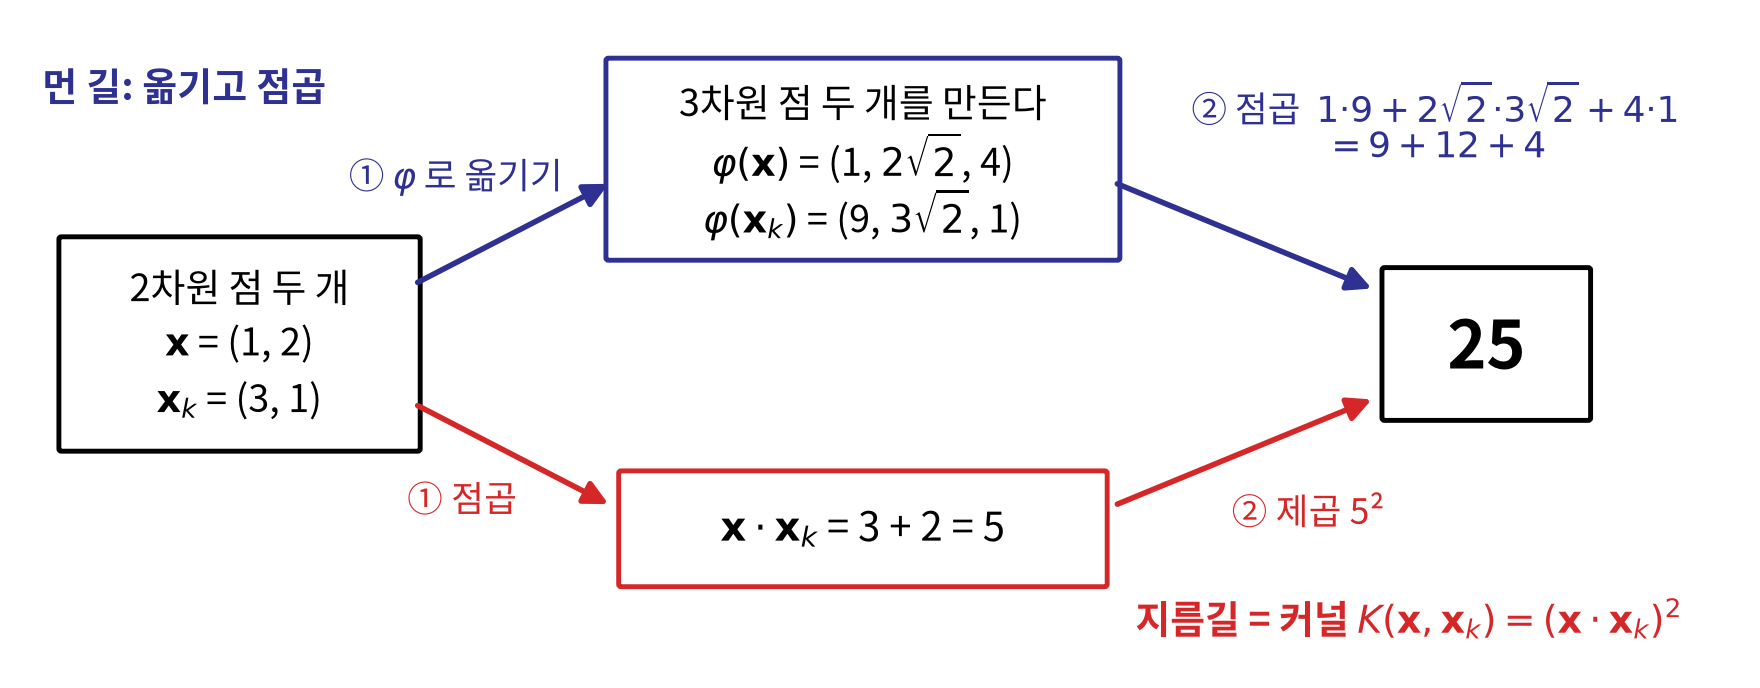
\includegraphics[width=0.65\linewidth]{kn_ktrick.png}\par\vskip0.1em
{\large $D(\mathbf{x}) = b + \sum_{k} \alpha_k y_k\, \mathbf{x}\cdot\mathbf{x}_k$ \;$\to$\; $D(\mathbf{x}) = b + \sum_{k} \alpha_k y_k\, \textcolor{ksablue}{\boldsymbol{K}(\mathbf{x}, \mathbf{x}_k)}$}\\[0.3em]
{\normalsize $\textcolor{ksablue}{K(\mathbf{x}, \mathbf{x}_k)} = (\mathbf{x}\cdot\mathbf{x}_k)^2 = (x_1x_{k1} + x_2x_{k2})^2 = (x_1^2)(x_{k1}^2) + (\sqrt2\,x_1x_2)(\sqrt2\,x_{k1}x_{k2}) + (x_2^2)(x_{k2}^2)$}\\[0.15em]
{\normalsize $= \varphi(\mathbf{x})\cdot\varphi(\mathbf{x}_k)$, \quad $\varphi(\mathbf{x}) = (x_1^2,\ \sqrt2\,x_1x_2,\ x_2^2)$ \;$\to$\; 옮긴 뒤의 점곱을 옮기지 않고 \kb{지름길}로}\\[0.15em]
{\small $\alpha$ 를 구하는 학습 식에도 점은 $\mathbf{x}_k\cdot\mathbf{x}_l$ 점곱으로만 나온다 \;$\to$\; 학습도 $K$ 로}
\vfill
\note{분류 식에서 점곱 자리에 다른 함수 K를 넣은 것이 커널 SVM입니다. 알파를 구하는 학습 식도, 라그랑주 식에 w를 대입해 정리하면 학습 점끼리의 점곱 x k 점곱 x l로만 쓰입니다. 그래서 학습할 때도 그 자리에 K를 넣으면 됩니다. 이 K를 커널이라고 부릅니다. 커널은 점들을 높은 차원으로 옮긴 뒤의 점곱을, 실제로 옮기지 않고 원래 점으로 바로 계산하는 함수입니다. 순서를 바꿔도 값이 같고, 두 점이 가까울수록 큰 값을 내서 유사도처럼 읽을 수 있습니다. 예를 들어 K를 점곱의 제곱으로 정해 봅시다. 점곱 x1 x k1 더하기 x2 x k2를 제곱해 펼치면 세 항이 나옵니다. x1 제곱 곱하기 x k1 제곱, 2 x1 x2 x k1 x k2, x2 제곱 곱하기 x k2 제곱입니다. 가운데 2를 루트2 두 개로 나눠 양쪽에 하나씩 주면, 세 항 모두 x 쪽 하나와 x k 쪽 하나의 곱이 됩니다. x 쪽만 모은 것이 파이 x, x1 제곱, 루트2 x1 x2, x2 제곱입니다. 그래서 점곱의 제곱은 이 3차원으로 옮긴 두 점의 점곱과 정확히 같습니다. 파이는 K를 펼쳐서 거꾸로 읽어 낸 것입니다. 이름은 앞 쪽 식에 맞춰 x는 새 점, x k는 서포트 벡터 같은 학습 점입니다. 그림의 위쪽 파란 길은 먼 길입니다. x 1, 2와 x k 3, 1을 각각 3차원 점 1, 2루트2, 4와 9, 3루트2, 1로 실제로 옮긴 뒤 점곱하면 1 곱하기 9, 2루트2 곱하기 3루트2, 4 곱하기 1입니다. 가운데는 2 곱하기 3이 6, 루트2 곱하기 루트2가 2라서 12입니다. 그래서 9 더하기 12 더하기 4, 25입니다. 아래쪽 빨간 길은 지름길입니다. 원래 점끼리 점곱하면 3 더하기 2, 5이고, 이것을 제곱하면 25입니다. 같은 값이 나오는데, 아래 길은 3차원 점을 만들지 않습니다. 이 지름길 함수, 점곱의 제곱이 커널 K입니다. 앞 쪽 식의 x 점곱 x k 자리에 K를 넣으면 커널 SVM입니다. 원 논문 식 4와 18이 바로 이 꼴입니다. 특징이 수천 개로 늘어나도 원래 점곱 하나로 계산하니, 특징을 직접 만드는 것보다 훨씬 가볍습니다. 이것이 커널 트릭입니다.}
\end{frame}

% --- 자주 쓰는 커널
\begin{frame}{자주 쓰는 커널}
\vfill
\centering
\renewcommand{\arraystretch}{1.35}
{\large\begin{tabular}{l|l}
선형 & $\langle \mathbf{x}, \mathbf{x}' \rangle$\\
다항 & $(\langle \mathbf{x}, \mathbf{x}' \rangle + 1)^q$\\
RBF & $\exp\!\big(-\gamma \lVert \mathbf{x}-\mathbf{x}' \rVert^2\big)$
\end{tabular}}\\[0.5em]
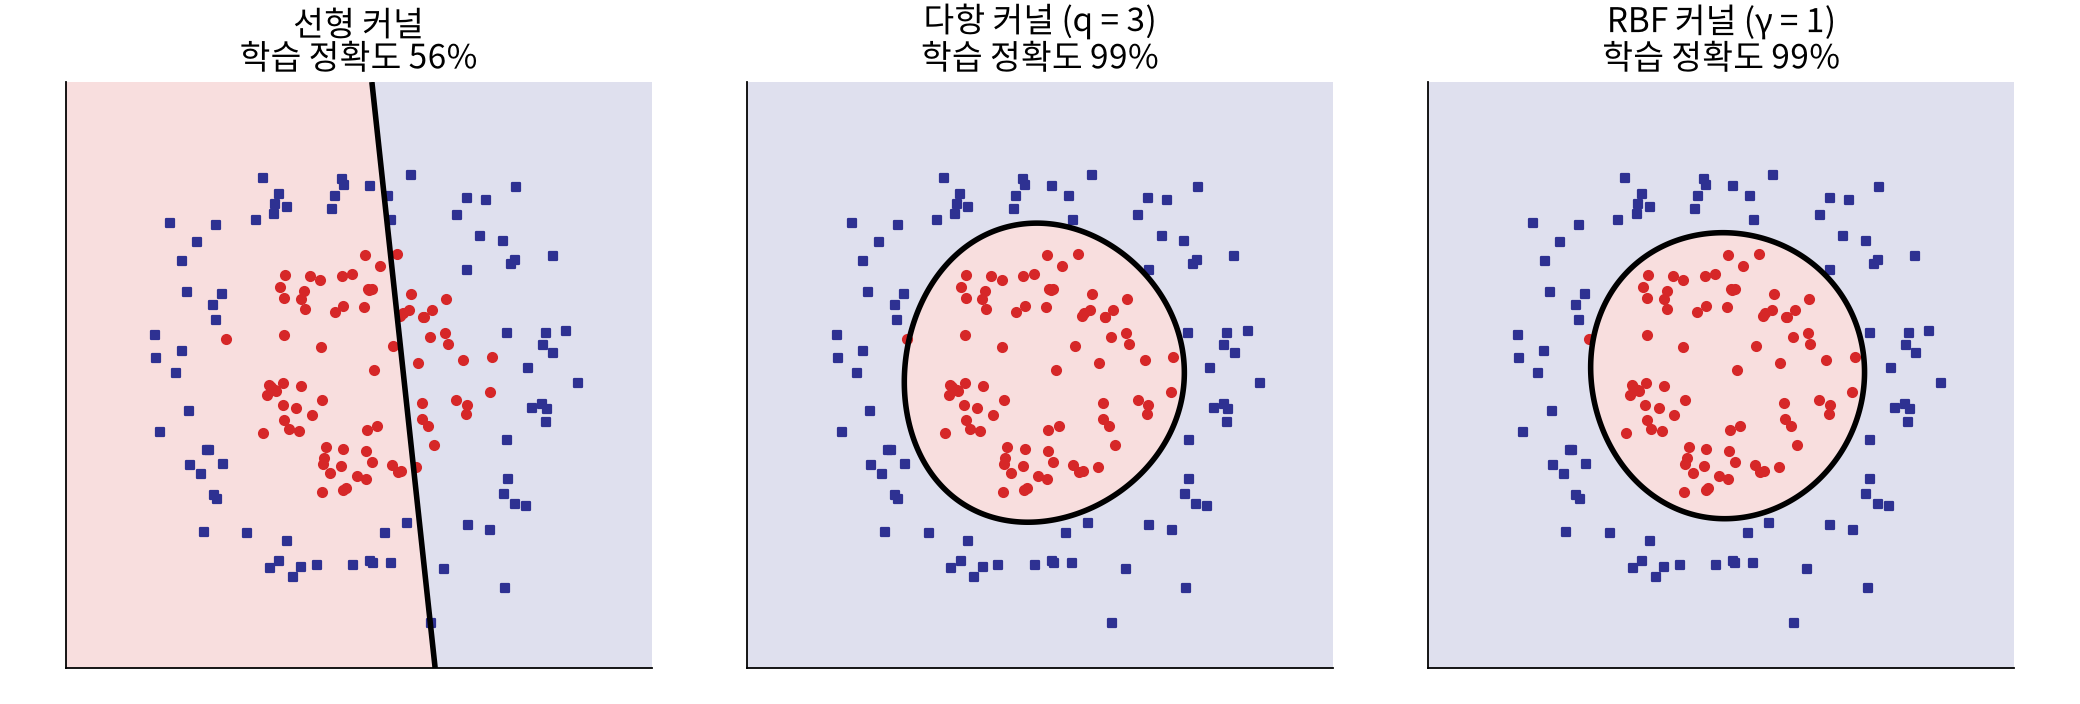
\includegraphics[width=0.8\linewidth]{sv_kernels.png}
\vfill
\note{자주 쓰는 커널은 세 가지입니다. 선형 커널은 그냥 점곱이라 앞의 서포트 벡터 분류기와 같습니다. 다항 커널은 점곱 더하기 1을 q제곱한 것으로, q차까지의 모든 곱을 특징으로 넣은 것과 같습니다. 차수를 q로 쓰는 것은 원 논문의 표기입니다. RBF 커널은 두 점 사이 거리의 제곱에 마이너스 감마를 곱해 지수를 취한 것으로, 학습 점마다 언덕을 하나씩 세워 그 높이를 특징으로 쓴 것과 같습니다. 다음 쪽 표에서 정리합니다. 아래 그림은 같은 원 모양 데이터에 세 커널을 쓴 결과입니다. 선형 커널은 직선이라 56퍼센트밖에 못 맞히고, q가 3인 다항 커널과 감마가 1인 RBF 커널은 원 모양 경계를 만들어 99퍼센트를 맞힙니다. 세 그림 모두 C는 1입니다.}
\end{frame}

% --- 세 커널 한눈에
\begin{frame}{선형 · 다항 · RBF 한눈에: 특징이 몇 개인가}
\markpage{kernels3}
\vfill
\centering
\renewcommand{\arraystretch}{1.2}
{\normalsize\begin{tabular}{c|c|c|c}
 & \textbf{선형} & \begin{tabular}{@{}c@{}}\textbf{다항} ($q = 2$)\\[-0.3em] {\small \kq{$+1$} $\to$ 0차 · 1차 항도}\end{tabular} & \textbf{RBF}\\ \hline
$K(\mathbf{x}, \mathbf{x}')$ & $\mathbf{x}\cdot\mathbf{x}'$ & $(\mathbf{x}\cdot\mathbf{x}' + 1)^2$ & $e^{-\gamma\lVert\mathbf{x}-\mathbf{x}'\rVert^2}$\\
특징 $\varphi(\mathbf{x})$ & $x_1,\ x_2$ & $1,\ x_1,\ x_2,\ x_1^2,\ x_1x_2,\ x_2^2$ & \begin{tabular}{@{}c@{}}$1,\ x_1,\ x_2,\ x_1^2,\ x_1x_2,\ x_2^2,$\\ $x_1^3,\ x_1^2x_2,\ x_1x_2^2,\ x_2^3,\ x_1^4,\ \dots$\end{tabular}\\
특징 수 $N$ & 2 & 6 & \kq{$\infty$}\\
특징 직접 만들기 & 된다 & 된다 & \kq{못 한다} $\to$ \kb{커널로만}\\
경계 & 직선 & 원 · 타원 · 쌍곡선 & 어떤 모양이든\\ \hline
실제 계산 & \multicolumn{3}{c}{셋 다 $D(\mathbf{x}) = b + \sum_{k} \alpha_k y_k K(\mathbf{x}, \mathbf{x}_k)$ \;(학습 점 $p$ 개 중 서포트 벡터만)}\\ \hline
\multicolumn{4}{c}{앞의 $(x_1,\ x_2,\ x_1^2 + x_2^2)$ = 다항 2차 특징 6개 중 일부를 손으로 고른 것}
\end{tabular}}\\[0.4em]
{\small 실제 상수: 다항은 $(1, \sqrt2 x_1, \sqrt2 x_2, x_1^2, \sqrt2 x_1x_2, x_2^2)$ 이어야 점곱이 $(\mathbf{x}\cdot\mathbf{x}' + 1)^2$ 과 정확히 같다\\ RBF 는 항마다 $e^{-\gamma\lVert\mathbf{x}\rVert^2}$ 와 차수별 상수가 곱해진다}
\vfill
\note{세 커널이 헷갈리니 한 표로 정리합니다. 기준은 하나, 특징을 몇 개 쓰는가입니다. 선형 커널은 특징을 늘리지 않습니다. x1, x2 그대로, 2개이고 경계는 직선입니다. 다항 커널 2차는 점곱 더하기 1을 제곱한 것인데, 앞의 지름길 예와 달리 더하기 1이 있어서 0차, 1차 항도 생깁니다. 펼쳐 보면 1, x1, x2, x1 제곱, x1 x2, x2 제곱, 이렇게 6개 특징의 점곱과 정확히 같습니다. 정확히는 루트2 같은 상수가 붙습니다. 이 6개로 직선을 그으면 원래 평면에서는 원, 타원, 쌍곡선 같은 2차 곡선이 됩니다. 앞에서 원 데이터에 높이 x1 제곱 더하기 x2 제곱을 붙였던 것은 커널이 아니라, 이 6개 중 몇 개를 손으로 골라 만든 특징 3개입니다. 그래서 원만 그릴 수 있었습니다. RBF는 펼치면 1, x1, x2, 2차 항 셋, 그다음 x1 세제곱, x1 제곱 x2, x1 x2 제곱, x2 세제곱, 4차 항, 이렇게 차수가 끝없이 이어져 특징이 무한 개입니다. 항마다 e의 마이너스 감마 x 길이 제곱과 차수별 상수가 곱해지지만 모양은 다항식 항 그대로입니다. 무한 개라 직접 만들 수는 없습니다. 그래서 맨 아래 줄이 중요합니다. 세 커널 모두 SVM이 실제로 계산하는 것은 똑같이 b 더하기 서포트 벡터마다 알파 곱하기 y 곱하기 K입니다. 특징 공간이 2차원이든 6차원이든 무한 차원이든, 계산은 학습 점 p개 중 서포트 벡터 수만큼의 K 값으로 끝납니다. 이것이 커널 트릭입니다. 특징 수와 계산하는 항의 수는 다른 것입니다. 언덕의 폭은 감마 하나로 모두 같고, 학습은 언덕마다 높이 알파를 정하는 것이며, 대부분 0이 되어 서포트 벡터의 언덕만 남습니다. 그래서 경계는 어떤 모양이든 될 수 있습니다. 감마는 언덕 폭이지 특징 수가 아닙니다.}
\end{frame}

% --- 다항 커널 전개
\begin{frame}{왜 $(\mathbf{x}\cdot\mathbf{x}' + 1)^2$ 가 특징 6개의 점곱인가}
\vfill
\centering
\renewcommand{\arraystretch}{1.4}
{\normalsize\begin{tabular}{rl}
\textbf{1.} & 점곱 풀기: \; $\mathbf{x}\cdot\mathbf{x}' = x_1x_1' + x_2x_2'$\\
\textbf{2.} & 제곱 펼치기: \; $(x_1x_1' + x_2x_2' + 1)^2$\\
 & $= 1 + 2x_1x_1' + 2x_2x_2' + x_1^2x_1'^2 + 2x_1x_2x_1'x_2' + x_2^2x_2'^2$\\
\textbf{3.} & 항마다 ($\mathbf{x}$ 쪽) $\times$ ($\mathbf{x}'$ 쪽) 로 나누기:\\
 & $1{\cdot}1 + (\sqrt2x_1)(\sqrt2x_1') + (\sqrt2x_2)(\sqrt2x_2') + (x_1^2)(x_1'^2) + (\sqrt2x_1x_2)(\sqrt2x_1'x_2') + (x_2^2)(x_2'^2)$\\
\textbf{4.} & $\mathbf{x}$ 쪽만 모으면: \; $\varphi(\mathbf{x}) = (1,\ \sqrt2x_1,\ \sqrt2x_2,\ x_1^2,\ \sqrt2x_1x_2,\ x_2^2)$ \;$\to$ \kb{6개}, \; $K = \varphi(\mathbf{x})\cdot\varphi(\mathbf{x}')$
\end{tabular}}\\[0.7em]
{\large 예: $\mathbf{x} = (1, 2)$, $\mathbf{x}' = (3, 1)$ \quad $(5 + 1)^2 = 36$ \; $=$ \; $1 + 6 + 4 + 9 + 12 + 4$}
\vfill
\note{다항 커널이 왜 특징 6개의 점곱과 같은지 직접 펼쳐 봅시다. 첫째, 점곱은 x1 x1 프라임 더하기 x2 x2 프라임입니다. 둘째, 이것에 1을 더해 제곱해서 펼치면 여섯 항이 나옵니다. 1, 2 x1 x1 프라임, 2 x2 x2 프라임, x1 제곱 x1 프라임 제곱, 2 x1 x2 x1 프라임 x2 프라임, x2 제곱 x2 프라임 제곱. 셋째, 각 항을 x에만 관한 것과 x 프라임에만 관한 것의 곱으로 나눕니다. 2 x1 x1 프라임은 루트2 x1 곱하기 루트2 x1 프라임입니다. 2는 루트2 두 개로 나눠 양쪽에 하나씩 줍니다. 넷째, x 쪽만 모으면 1, 루트2 x1, 루트2 x2, x1 제곱, 루트2 x1 x2, x2 제곱, 6개의 특징이 되고, 커널 값은 이 6개짜리 벡터 두 개의 점곱과 정확히 같습니다. 숫자로 확인하면 x가 1, 2이고 x 프라임이 3, 1일 때 점곱은 5, 5 더하기 1의 제곱은 36입니다. 6개 특징으로 계산해도 1 더하기 6 더하기 4 더하기 9 더하기 12 더하기 4, 36입니다. 커널은 이 6개를 만들지 않고 점곱 하나, 덧셈 하나, 제곱 하나로 같은 값을 냅니다.}
\end{frame}

% --- RBF 전개
\begin{frame}{RBF 를 $x$ 로 쓰면: 특징이 끝없이 나온다}
\vfill
\centering
{\normalsize 가장 쉬운 경우: 특징 1개 ($x$ 하나), $\gamma = \tfrac12$}\\[0.3em]
\renewcommand{\arraystretch}{2.0}
{\normalsize\begin{tabular}{rl}
\textbf{1.} & 거리 풀기: \; $e^{-(x - x')^2/2} = e^{-x^2/2}\; e^{-x'^2/2}\; e^{\,x x'}$\\
\textbf{2.} & 테일러: \; $e^{\,x x'} = 1 + x x' + \dfrac{(x x')^2}{2!} + \dfrac{(x x')^3}{3!} + \cdots$ \quad (끝이 없다)\\
\textbf{3.} & 항마다 ($x$ 쪽) $\times$ ($x'$ 쪽): \; $\dfrac{(x x')^q}{q!} = \dfrac{x^q}{\sqrt{q!}} \cdot \dfrac{x'^q}{\sqrt{q!}}$\\
\textbf{4.} & $x$ 쪽만 모으면: \; $\varphi(x) = e^{-x^2/2}\Big(1,\ x,\ \dfrac{x^2}{\sqrt{2!}},\ \dfrac{x^3}{\sqrt{3!}},\ \cdots\Big)$ \;$\to$ \kq{끝없이} $= \infty$ 개
\end{tabular}}\\[0.5em]
{\normalsize 특징이 2개 ($x_1, x_2$) 면: \; $1,\ x_1,\ x_2,\ x_1^2,\ x_1x_2,\ x_2^2,\ x_1^3,\ x_1^2x_2,\ \cdots$ \; \kb{차수가 끝없이}}\\[0.3em]
{\large 특징 $\infty$ 개는 만들 수 없다 $\to$ RBF 는 \kq{커널 트릭으로만} 쓸 수 있다}
\vfill
\note{이번엔 RBF를 x로 직접 써 봅시다. 가장 쉽게, 특징이 x 하나뿐이고 감마가 2분의 1인 경우입니다. 첫째, x 빼기 x 프라임의 제곱을 풀면 x 제곱 더하기 x 프라임 제곱 빼기 2 x x 프라임이라, RBF는 e의 마이너스 x 제곱 나누기 2, e의 마이너스 x 프라임 제곱 나누기 2, 그리고 e의 x x 프라임 승, 세 개의 곱입니다. 둘째, 마지막 것을 테일러 급수로 펼치면 1 더하기 x x 프라임 더하기 x x 프라임 제곱 나누기 2 팩토리얼, 이렇게 끝없이 이어집니다. 셋째, 다항 커널 때처럼 각 항을 x 쪽과 x 프라임 쪽의 곱으로 나눕니다. x x 프라임의 q제곱 나누기 q 팩토리얼은 x의 q제곱 나누기 루트 q 팩토리얼 곱하기 x 프라임의 q제곱 나누기 루트 q 팩토리얼입니다. 넷째, x 쪽만 모으면 특징은 1, x, x 제곱 나누기 루트2, x 세제곱 나누기 루트6, 이렇게 끝없이 이어지고, 전체에 e의 마이너스 x 제곱 나누기 2가 곱해집니다. 다항 커널은 제곱에서 끝나서 항이 6개였는데, RBF는 테일러 급수가 끝나지 않아서 특징이 무한 개입니다. 특징이 x1, x2 두 개면 1, x1, x2, x1 제곱, x1 x2, x2 제곱, x1 세제곱, 이렇게 모든 차수의 항이 다 나옵니다. 숫자로 확인해 봅시다. x가 1, x 프라임이 0.5면 RBF 값은 e의 마이너스 0.125, 0.8825입니다. 특징을 1개만 쓰면 0.54, 2개면 0.80, 3개면 0.87, 4개면 0.881, 6개면 0.8825로 점점 정확한 값에 다가갑니다. 무한 개를 다 만들 수는 없으니, 커널은 이 값을 e의 마이너스 감마 거리 제곱 한 번으로 바로 계산합니다. 그래서 RBF는 다항 커널과 달리 특징을 직접 만들어 선형 SVM을 돌리는 방법이 원리상 불가능합니다. 특징이 무한 개라 만들 수가 없기 때문입니다. 커널 트릭이 있어야만 쓸 수 있는 방법이고, 커널 트릭이 왜 필요한지 가장 잘 보여 주는 예입니다. 참고로 무한 개를 유한 개, 예를 들어 500개로 흉내 내는 근사는 있습니다. sklearn의 RBFSampler, Nystroem이 그것이고, 데이터가 아주 클 때 이렇게 만든 특징으로 선형 SVM을 돌리기도 합니다. 하지만 정확한 RBF SVM은 커널로만 됩니다.}
\end{frame}

% --- 방법 A vs B
\begin{frame}{특징을 직접 만들기 vs 커널: 같은 경계}
\vfill
\centering
\renewcommand{\arraystretch}{1.5}
{\normalsize\begin{tabular}{l|c|c}
 & \textbf{A. 특징 직접 만들기} & \textbf{B. 커널} \\ \hline
점을 바꾸나 & $\varphi(\mathbf{x})$ 6개를 \kb{만든다} & \kq{안 만든다}\\
$K$ 를 쓰나 & 안 쓴다 ($\varphi$ 끼리 그냥 점곱) & $K(\mathbf{x}, \mathbf{x}') = (\mathbf{x}\cdot\mathbf{x}' + 1)^2$\\
학습하는 것 & $\mathbf{w}$ (\kb{특징마다} 하나): 6개 & $\alpha$ (\kq{점마다} 하나): 120개, 0 아닌 것 21개\\
분류기 & $\sum_{i=1}^{N} w_i\varphi_i(\mathbf{x}) + b$ & $b + \sum_k \alpha_k y_k K(\mathbf{x}, \mathbf{x}_k)$\\ \hline
원 120개 & \multicolumn{2}{c}{둘 다 $\mathbf{w} = (0,\ 0.11,\ 0.13,\ -2.81,\ 0.02,\ -3.09)$, $b = 1.64$ \;(예측도 모두 같다)}
\end{tabular}}\\[0.6em]
{\large 잇는 식: \; $\mathbf{w} = \sum_k \alpha_k y_k\, \varphi(\mathbf{x}_k)$ \qquad $K(\mathbf{x}, \mathbf{x}') = \varphi(\mathbf{x})\cdot\varphi(\mathbf{x}')$}\\[0.4em]
{\normalsize 다항 2차: A · B 둘 다 된다 \quad RBF: $\varphi$ 가 \kq{$\infty$} 개라 A 는 처음부터 불가능 $\to$ \kb{커널 트릭으로만} 된다}
\vfill
\note{같은 다항 2차 경계를 만드는 방법이 두 가지입니다. A는 특징을 직접 만드는 방법입니다. 점마다 1, 루트2 x1, 루트2 x2, x1 제곱, 루트2 x1 x2, x2 제곱, 숫자 6개를 실제로 만들고, 지난 시간의 평범한 선형 SVM으로 w 6개를 학습합니다. 여기에는 커널 K가 나오지 않습니다. 앞의 원 데이터에 높이를 붙인 것도 A입니다. B는 커널입니다. 특징을 만들지 않고, 두 점마다 점곱 더하기 1의 제곱, K만 계산해서 학습 점마다 하나씩 알파를 학습합니다. 원 데이터 120개로 실제로 해 보면, B의 알파는 120개이고 0이 아닌 것이 21개, 서포트 벡터입니다. 이 알파로 w를 계산하면, 아래 식 w는 알파 k 곱하기 y k 곱하기 파이 x k의 합, 원 논문 식 6이고, A가 학습한 w 6개와 소수 셋째 자리까지 똑같고 b도 1.64로 같습니다. 120개 점의 예측도 모두 같습니다. 두 방법을 잇는 것은 K가 파이끼리의 점곱이라는 식입니다. 다항 2차처럼 특징이 6개뿐이면 A로 해도 됩니다. 그런데 차수가 높거나 원래 특징이 많으면 A의 특징 수가 폭발하고, RBF는 특징이 무한 개라 A가 아예 불가능합니다. 그래서 B, 커널을 씁니다. 이것이 커널 트릭입니다.}
\end{frame}

% --- RBF 커널 자세히
\begin{frame}{RBF 커널: 거리로 재는 가까움 점수}
\vfill
\centering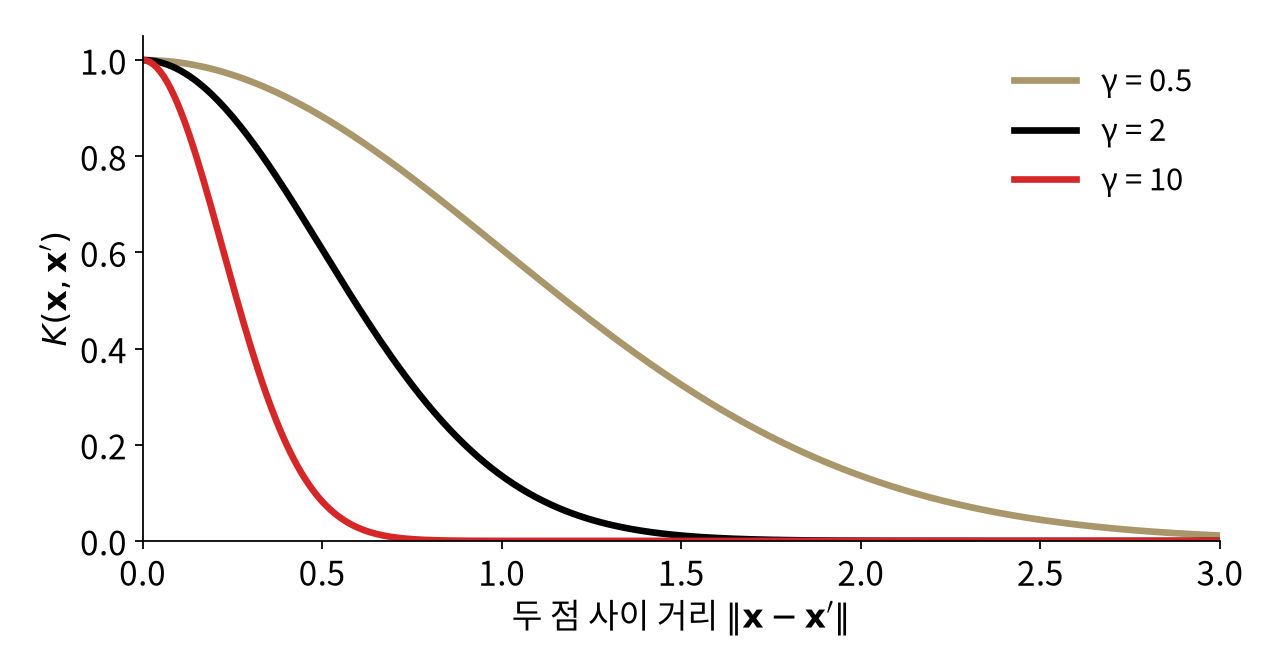
\includegraphics[width=0.62\linewidth]{sv_rbf.png}\par\vskip0.2em
{\large $K(\mathbf{x}, \mathbf{x}') = e^{-\gamma\lVert\mathbf{x}-\mathbf{x}'\rVert^2}$: 두 점이 같으면 \kb{1}, 멀면 \kb{0}}\\[0.3em]
{\normalsize $\gamma$ 가 크면 조금만 멀어져도 0 \quad ($\mathbf{x}'$ 를 중심으로 한 \kb{언덕} 하나)}
\vfill
\note{RBF 커널을 자세히 봅시다. RBF 커널은 두 점 사이 거리의 제곱에 마이너스 감마를 곱해 e의 지수로 올린 것입니다. 같은 점이면 거리가 0이라 1, 멀어질수록 0으로 떨어지는 가까움 점수입니다. 감마가 크면 조금만 멀어져도 금방 0이 되고, 작으면 멀리까지 1에 가깝게 남습니다. 대략 1 나누기 루트 감마 정도의 거리까지 영향이 미친다고 보면 됩니다. 한 점 x 프라임을 고정하고 x를 움직이면, x 프라임 자리에서 1로 가장 높고 멀어질수록 0으로 내려가는 종 모양 언덕 하나가 됩니다. 다음 쪽부터 이 언덕으로 분류기를 만듭니다.}
\end{frame}

% --- 언덕 1개 vs 서포트 벡터마다 언덕
\begin{frame}{RBF 는 $(x_1, x_2, \text{높이 하나})$ 가 아니다}
\vfill
\centering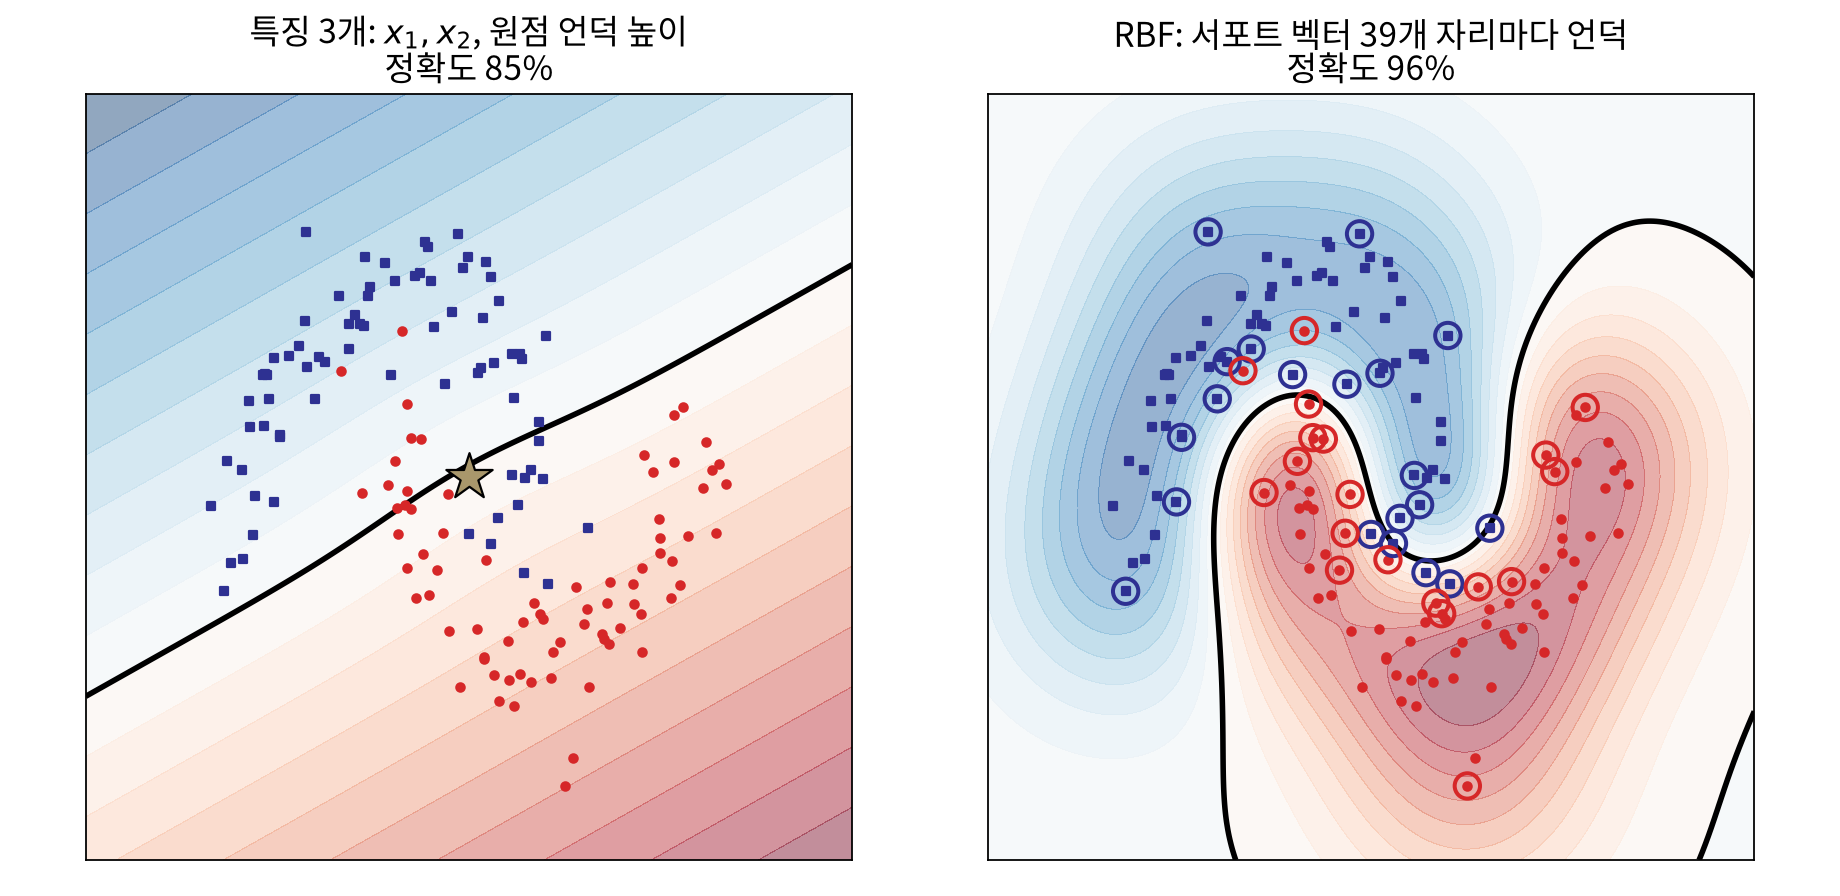
\includegraphics[width=0.72\linewidth]{sv_hills.png}\par\vskip0.2em
{\large 언덕 1개 $\to$ \kq{원 비슷한 경계만} \quad 서포트 벡터마다 언덕 (빨강 $+$, 파랑 $-$) $\to$ \kb{어떤 모양이든}}
\vfill
\note{헷갈리기 쉬운 부분입니다. 앞에서 원 모양 데이터에 높이 x1 제곱 더하기 x2 제곱을 붙여 특징 3개로 만들었습니다. 그러면 RBF도 x1, x2에 rbf 값 하나를 붙인 특징 3개일까요? 아닙니다. rbf는 점 하나로는 계산이 안 되고 기준점이 하나 더 필요합니다. 기준점을 원점 하나로 잡으면 원점에 세운 언덕 하나이고, 이것은 높이 x1 제곱 더하기 x2 제곱을 붙인 것과 같은 생각입니다. 왼쪽 그림이 반달 데이터에 그렇게 한 것입니다. 금색 별이 언덕의 중심입니다. 언덕 하나로 만들 수 있는 경계는 원 비슷한 모양뿐이라 85퍼센트에 그칩니다. RBF SVM은 오른쪽처럼 서포트 벡터마다, 동그라미 친 점마다 그 자리에 언덕을 하나씩 세우고, 빨간 서포트 벡터는 위로, 파란 서포트 벡터는 아래로 알파만큼 키워서 더합니다. 이 합이 배경색이고, 0인 곳이 검은 경계입니다. 언덕 39개를 겹치니 반달처럼 휘어진 경계도 만들어 96퍼센트를 맞힙니다. 감마는 1, C는 1입니다.}
\end{frame}

% --- RBF 피처 수
\begin{frame}{RBF 는 실제로 어떻게 계산하나: 학습 점마다 언덕 하나}
\vfill
\centering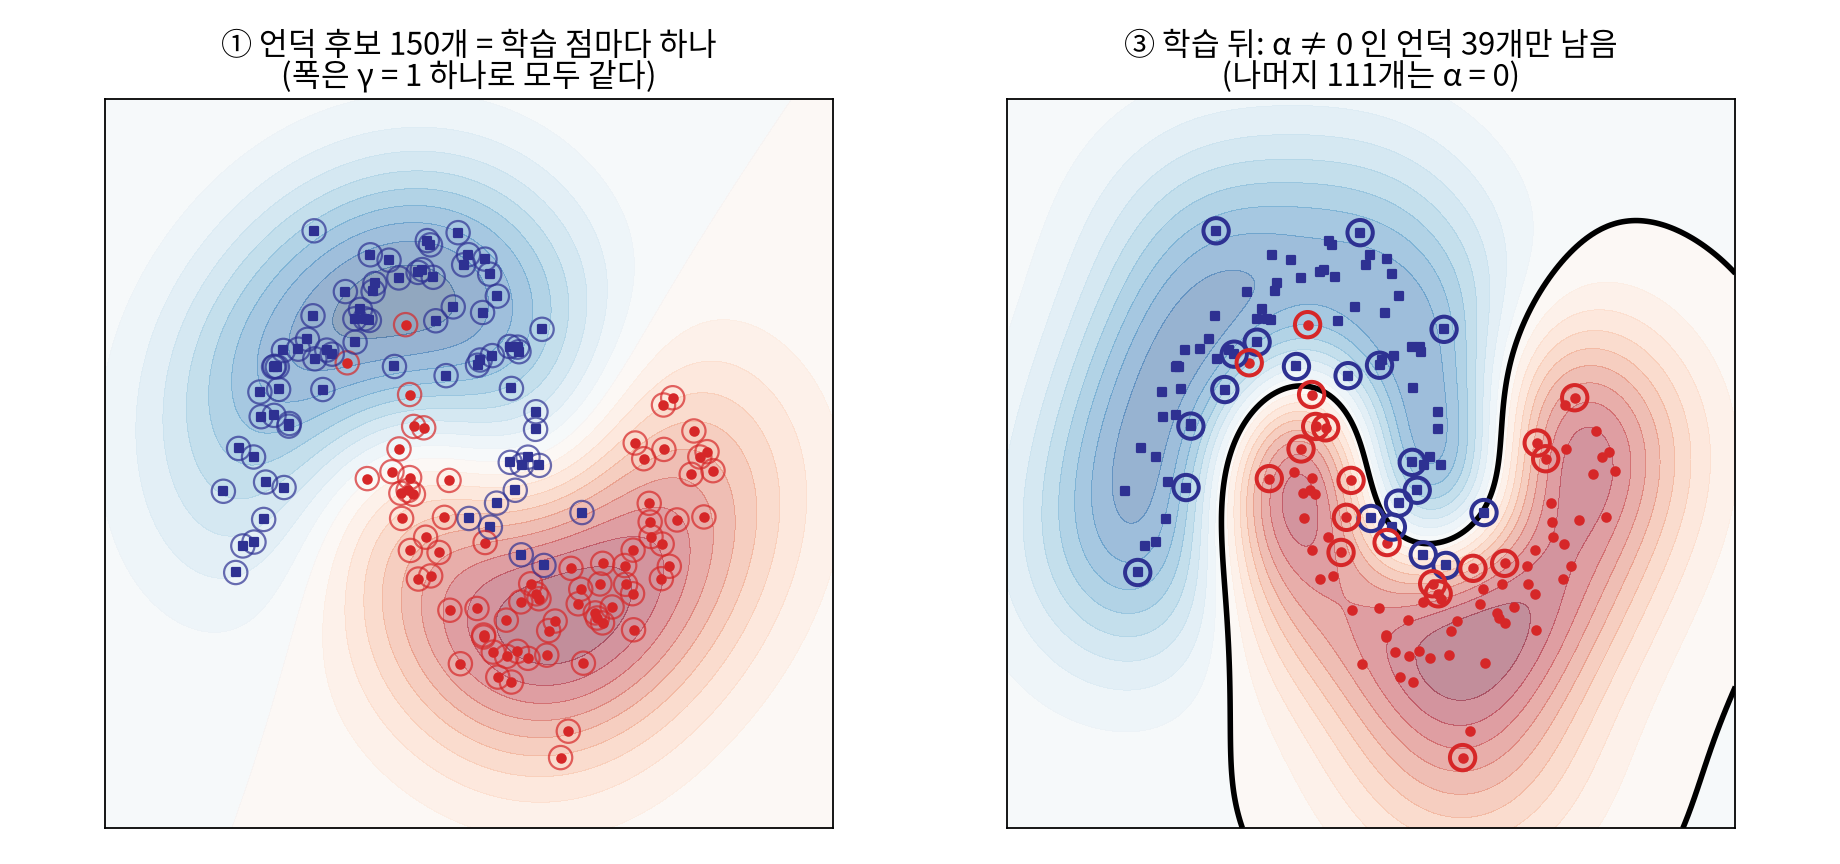
\includegraphics[width=0.56\linewidth]{sv_hill_count.png}\par\vskip0.3em
\renewcommand{\arraystretch}{1.25}
{\small\begin{tabular}{rl|rl}
\textbf{①} & 언덕 후보 = 점마다 1개 ($p = 150$), 폭 \kq{$\gamma$ 하나} &
\textbf{③} & 학습 = 높이 $\alpha_k$, 대부분 0 $\to$ \kb{39개} 남음\\
\textbf{②} & 새 점에서 언덕 150개 높이 $K(\mathbf{x}, \mathbf{x}_k)$ &
\textbf{④} & 예측 = $D(\mathbf{x}) = b + \sum_k \alpha_k y_k K$ 의 부호
\end{tabular}}\\[0.5em]
{\large 학습할 때: 언덕 후보 \kb{150개} (모든 학습 점) 다 본다 \quad 예측할 때: $\alpha_k \ne 0$ 인 \kb{39개}만 쓴다}
\vfill
\note{그러면 특징이 무한 개인 RBF를 실제로는 어떻게 계산할까요. 감마를 여러 개 쓰는 게 아닙니다. 감마는 하나이고, 학습 점마다 언덕을 하나씩 세웁니다. 단계별로 보겠습니다. 첫째, 반달 데이터는 점이 150개입니다. 점마다 그 자리를 중심으로 언덕을 하나씩 세워, 언덕 후보가 150개입니다. 중심은 다 다르고, 폭은 감마 하나로 모두 같습니다. 왼쪽 그림이 150개 언덕을 모두 같은 높이로 세운 것입니다. 둘째, 새 점 x가 오면 150개 언덕 각각에서 높이를 읽습니다. 어떤 학습 점 바로 옆이면 그 언덕 값은 1에 가깝고, 멀면 0입니다. 무한 개의 특징을 직접 만드는 대신, 학습 점 하나하나와 얼마나 가까운가, 이 150개 값으로 계산합니다. 셋째, 학습은 언덕마다 높이 알파를 정하는 것입니다. 빨간 점의 언덕은 위로, 파란 점의 언덕은 아래로입니다. SVM은 경계 근처 점만 알파가 0이 아니고, 나머지 111개는 알파가 0이 되어 언덕이 사라집니다. 남은 39개가 서포트 벡터이고, 오른쪽 그림이 그 39개 언덕을 알파만큼 키워 더한 것입니다. 넷째, 예측은 그 합 D의 부호이고, 0인 곳이 검은 경계입니다. 정리하면, 학습할 때는 150개 학습 점 모두를 언덕 후보로 놓고 알파를 정하고, 예측할 때는 알파가 0이 아닌 39개, 서포트 벡터의 언덕만 씁니다. 150개와 39개는 같은 이야기의 학습 전과 학습 후입니다. 감마는 특징 수가 아니라 언덕 폭입니다. 작으면 넓은 언덕이라 멀리까지 영향을 주어 경계가 매끈하고, 크면 좁은 언덕이라 점마다 섬이 생겨 과대적합됩니다. 감마는 학습으로 정하지 않고 교차 검증으로 하나 고릅니다. 이 150개 언덕 특징으로 로지스틱 회귀를 해도 비슷한 경계가 나오는데, SVM은 대부분의 알파를 0으로 만들어 언덕 몇 개만 남긴다는 점이 다릅니다.}
\end{frame}

% --- gamma
\begin{frame}{RBF 커널의 $\gamma$: 얼마나 구불구불하게}
\vfill
\centering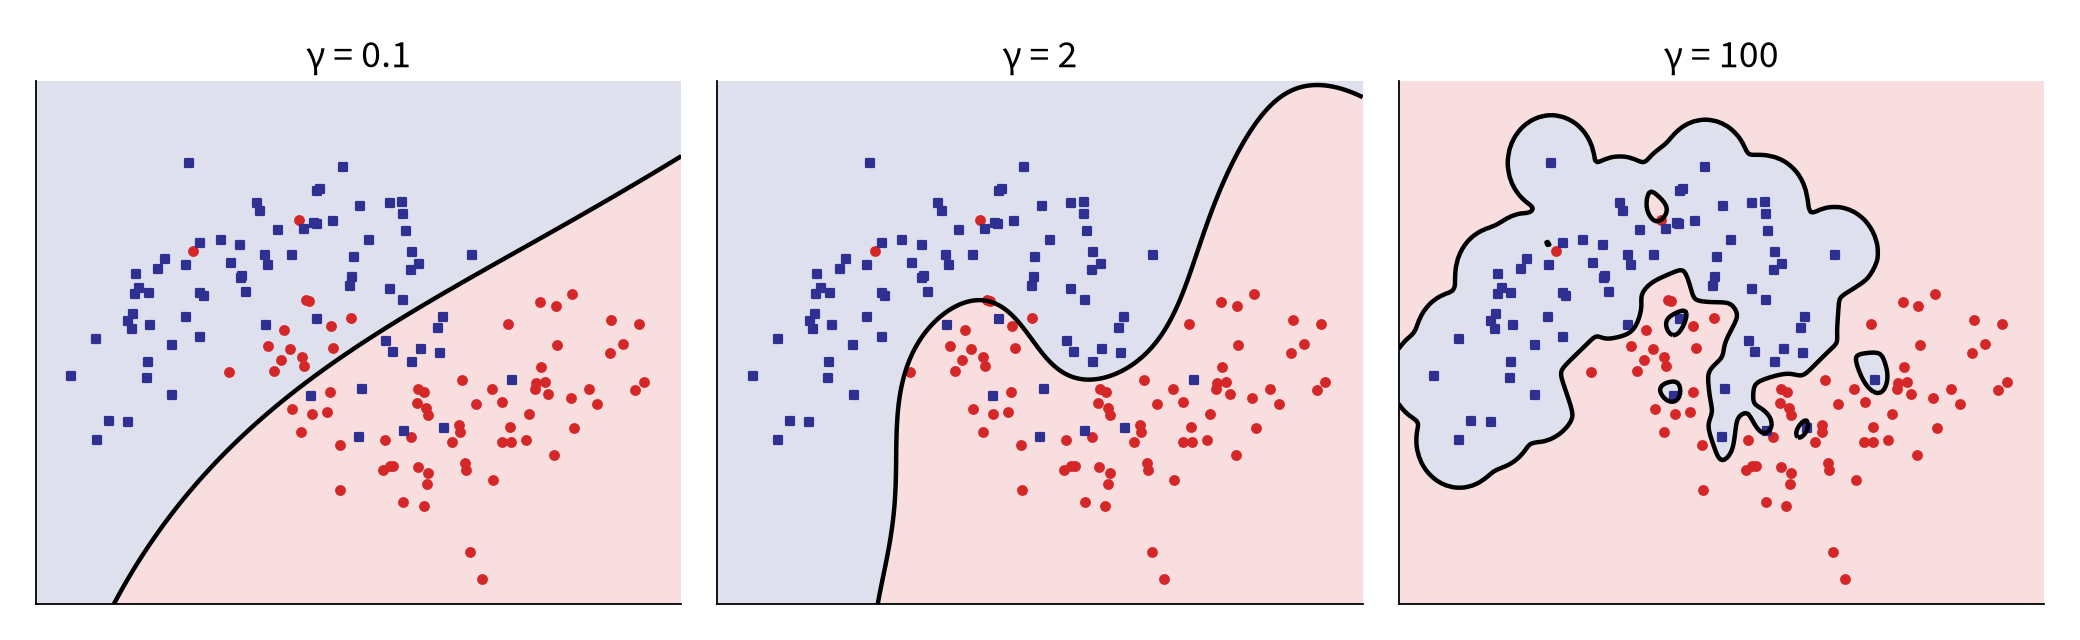
\includegraphics[width=0.92\linewidth]{sv_gamma.png}\par\vskip0.2em
{\large $\gamma$ 작으면 과소적합 \quad 크면 \kq{과대적합}}
\vfill
\note{RBF 커널의 감마는 앞 쪽의 언덕 폭, 점 하나의 영향이 얼마나 멀리까지 미치는지를 정합니다. 대략 1 나누기 루트 감마 거리까지입니다. 감마가 0.1로 작으면 영향이 넓게 퍼져서 경계가 거의 직선입니다. 반달 모양을 못 따라가는 과소적합입니다. 감마가 2면 반달을 따라 적당히 휘어집니다. 감마가 100이면 점 하나하나의 영향이 아주 좁아서 점마다 섬이 생깁니다. 학습 데이터를 외운 과대적합입니다. 그래서 SVM을 쓸 때는 C와 감마 두 숫자를 교차 검증으로 함께 고릅니다. 실습에서 직접 해 봅니다.}
\end{frame}

\section{정리}
% --- 장단점
\begin{frame}{SVM 정리: 장점과 단점}
\vfill
\centering
\renewcommand{\arraystretch}{1.6}
{\large\begin{tabular}{c|c}
{\Large\kb{장점}} & {\Large\kq{단점}}\\ \hline
볼록 최적화 $\to$ 답이 \textbf{하나} & $C$ · 커널 · $\gamma$ 를 골라야 한다 (교차 검증)\\
$C$ 로 과대적합 조절 & 기본은 \textbf{두 클래스}용\\
커널로 경계 모양이 자유롭다 & 해석이 어렵다, 확률을 주지 않는다\\
예측엔 서포트 벡터만 필요 & 데이터가 아주 많으면 학습이 느리다
\end{tabular}}
\vfill
\note{정리하면 SVM의 장점은 첫째, 볼록 최적화 문제라 답이 하나로 정해지고 시작점에 따라 달라지지 않습니다. 둘째, C로 과대적합을 조절할 수 있습니다. 셋째, 커널을 바꿔 경계 모양을 자유롭게 만들 수 있습니다. 넷째, 예측할 때 서포트 벡터만 있으면 됩니다. 단점은 C, 커널, 감마 같은 숫자를 교차 검증으로 골라야 하고, 기본적으로 두 클래스를 가르는 방법이며, 로지스틱회귀처럼 확률을 주지 않고 왜 그렇게 분류했는지 해석하기 어렵다는 점입니다. 데이터가 많으면 커널 SVM의 학습이 느려지는 것도 단점입니다. 이유는 커널이 두 점씩 짝으로 계산되기 때문입니다. 학습할 때는 원칙적으로 모든 짝의 K가 필요해서, 점이 1만 개면 1만 곱하기 1만, 1억 개이고 다 저장하면 약 800메가바이트입니다. sklearn은 이 표를 한꺼번에 만들지 않고 두 점씩 고쳐 가며 필요한 줄만 그때그때 계산하지만, 그래도 학습 시간이 점 수의 제곱 이상으로 늘어 수만 개를 넘으면 현실적이지 않습니다. 예측할 때는 서포트 벡터만 쓰니 그 수만큼만 K를 계산합니다. 데이터가 크면 커널 없는 선형 SVM을 쓰거나, RBF 특징을 수백 개로 근사해 만드는 방법, 예를 들어 sklearn의 Nystroem이나 RBFSampler를 쓰거나, 트리 부스팅이나 신경망 같은 다른 모델을 씁니다. RBF SVM이 잘 맞는 것은 실습의 지폐 데이터 1,372개처럼 수천에서 수만 개 정도의 데이터입니다.}
\end{frame}

\section{연습}
% --- 실습
\begin{frame}{실습}
\vfill
\centering\begin{tabular}{rl}
\large 1 & 원 데이터: 특징 6개 직접 만들기 (A) vs 다항 커널 (B) 가 같은 $\mathbf{w}$ 인지 확인\\[0.5em]
\large 2 & 실제 데이터: 지폐 1,372장 진위 판별, 선형 vs RBF\\[0.5em]
\large 3 & 반달 데이터에서 $C$ 와 $\gamma$ 를 교차 검증으로 고르기
\end{tabular}\vskip1em
Banknote Authentication (Lohweg; UCI) \\[0.4em]\href{https://colab.research.google.com/github/SuminHan/book-ml/blob/main/slides/ml1/week03/1_svm_kernel/lab/svm_kernel.ipynb}{\textcolor{ksagolddk}{▶ Colab에서 실습 노트북 열기}}
\vfill
\note{실습은 세 부분입니다. 첫째, 원 데이터에서 특징 6개를 직접 만드는 방법과 다항 커널이 같은 w를 주는지 확인합니다. 둘째, 지폐 진위 데이터에서 선형과 RBF 커널을 비교합니다. 셋째, 반달 데이터에서 C와 감마를 교차 검증으로 고르고 경계를 그려 봅니다. sklearn의 C는 지난 시간에 본 벌점이라, 크면 좁은 길입니다.}
\end{frame}

% --- 정리
\begin{frame}{정리}
\vfill
\centering\normalsize\begin{tabular}{l}
\textbf{특징 늘리기}: 점에 숫자를 붙여 올리면, 올린 곳의 직선 = 원래 자리의 \kb{휘어진 경계}\\[0.5em]
\textbf{커널}: $K(\mathbf{x}, \mathbf{x}') = \varphi(\mathbf{x})\cdot\varphi(\mathbf{x}')$ 를 $\varphi$ 없이 바로 계산\\[0.5em]
\textbf{두 방법}: A 특징 직접 $\to$ $\mathbf{w}$ (특징마다) \;=\; B 커널 $\to$ $\alpha$ (점마다), \;$\mathbf{w} = \sum_k \alpha_k y_k \varphi(\mathbf{x}_k)$\\[0.5em]
\textbf{특징 수}: 선형 2 · 다항 2차 6 · RBF $\infty$ (그래서 RBF 는 커널로만)\\[0.5em]
\textbf{RBF}: 학습 점마다 언덕, 폭 $\gamma$ 하나, 예측엔 서포트 벡터의 언덕만\\[0.5em]
\textbf{$\gamma$}: 작으면 매끈 (과소적합), 크면 구불구불 (\kq{과대적합}) $\to$ 교차 검증
\end{tabular}
\vfill
\note{정리합니다. 점에 숫자, 즉 특징을 붙여 높은 차원으로 올리면, 올린 곳에서 직선으로 가르는 것이 원래 자리에서는 휘어진 경계가 됩니다. 커널은 올린 뒤의 점곱을, 올리지 않고 원래 점으로 바로 계산하는 함수입니다. 같은 경계를 만드는 방법이 둘인데, 특징을 직접 만들어 특징마다 w를 학습하는 것과, 커널로 점마다 알파를 학습하는 것이고, w는 알파 곱하기 y 곱하기 파이의 합이라 둘은 같은 경계입니다. 특징 수는 선형 2, 다항 2차 6, RBF는 무한이라 RBF는 커널로만 계산합니다. RBF는 학습 점마다 언덕을 세우고 폭은 감마 하나이며, 예측할 때는 서포트 벡터의 언덕만 씁니다. 감마가 작으면 매끈하고 크면 구불구불해서 과대적합되니 교차 검증으로 고릅니다.}
\end{frame}

\begin{frame}{참고 문헌}
\vfill
\small
\begin{itemize}
\setlength{\itemsep}{0.45em}
\item Boser, B. E., Guyon, I. M., \& Vapnik, V. N. (1992). A training algorithm for optimal margin classifiers. \textit{COLT '92}, 144--152. \;(커널 · RBF) \paperlink{https://doi.org/10.1145/130385.130401}
\item James, G., Witten, D., Hastie, T., \& Tibshirani, R. \textit{An Introduction to Statistical Learning}, 9장. \paperlink{https://doi.org/10.1007/978-1-0716-1418-1}
\item Wang, S. (2019). CME 250 Lecture 5: Support Vector Machines, Stanford. \paperlink{https://web.stanford.edu/class/cme250/files/cme250_lecture5.pdf}
\item 수학 고양이 (YouTube). 등산로 하나로 끝내는 라그랑주 승수법 풀코스. \;(라그랑주 · KKT, 15:25 부터) \paperlink{https://youtu.be/dIS9MtVzZCM?t=925}
\item 위키백과: 서포트 벡터 머신 \paperlink{https://ko.wikipedia.org/wiki/\%EC\%84\%9C\%ED\%8F\%AC\%ED\%8A\%B8_\%EB\%B2\%A1\%ED\%84\%B0_\%EB\%A8\%B8\%EC\%8B\%A0} \;·\; Kernel method \paperlink{https://en.wikipedia.org/wiki/Kernel_method}
\end{itemize}
\vfill
\note{이 덱의 참고 문헌입니다.}
\end{frame}
\end{document}
